\subsection{Particle 2}

\begin{figure}[ H]

\caption{Particle 2: $ \lambda: 13.9227$Depth: 30 out of $200 \mu $ m}

\centering

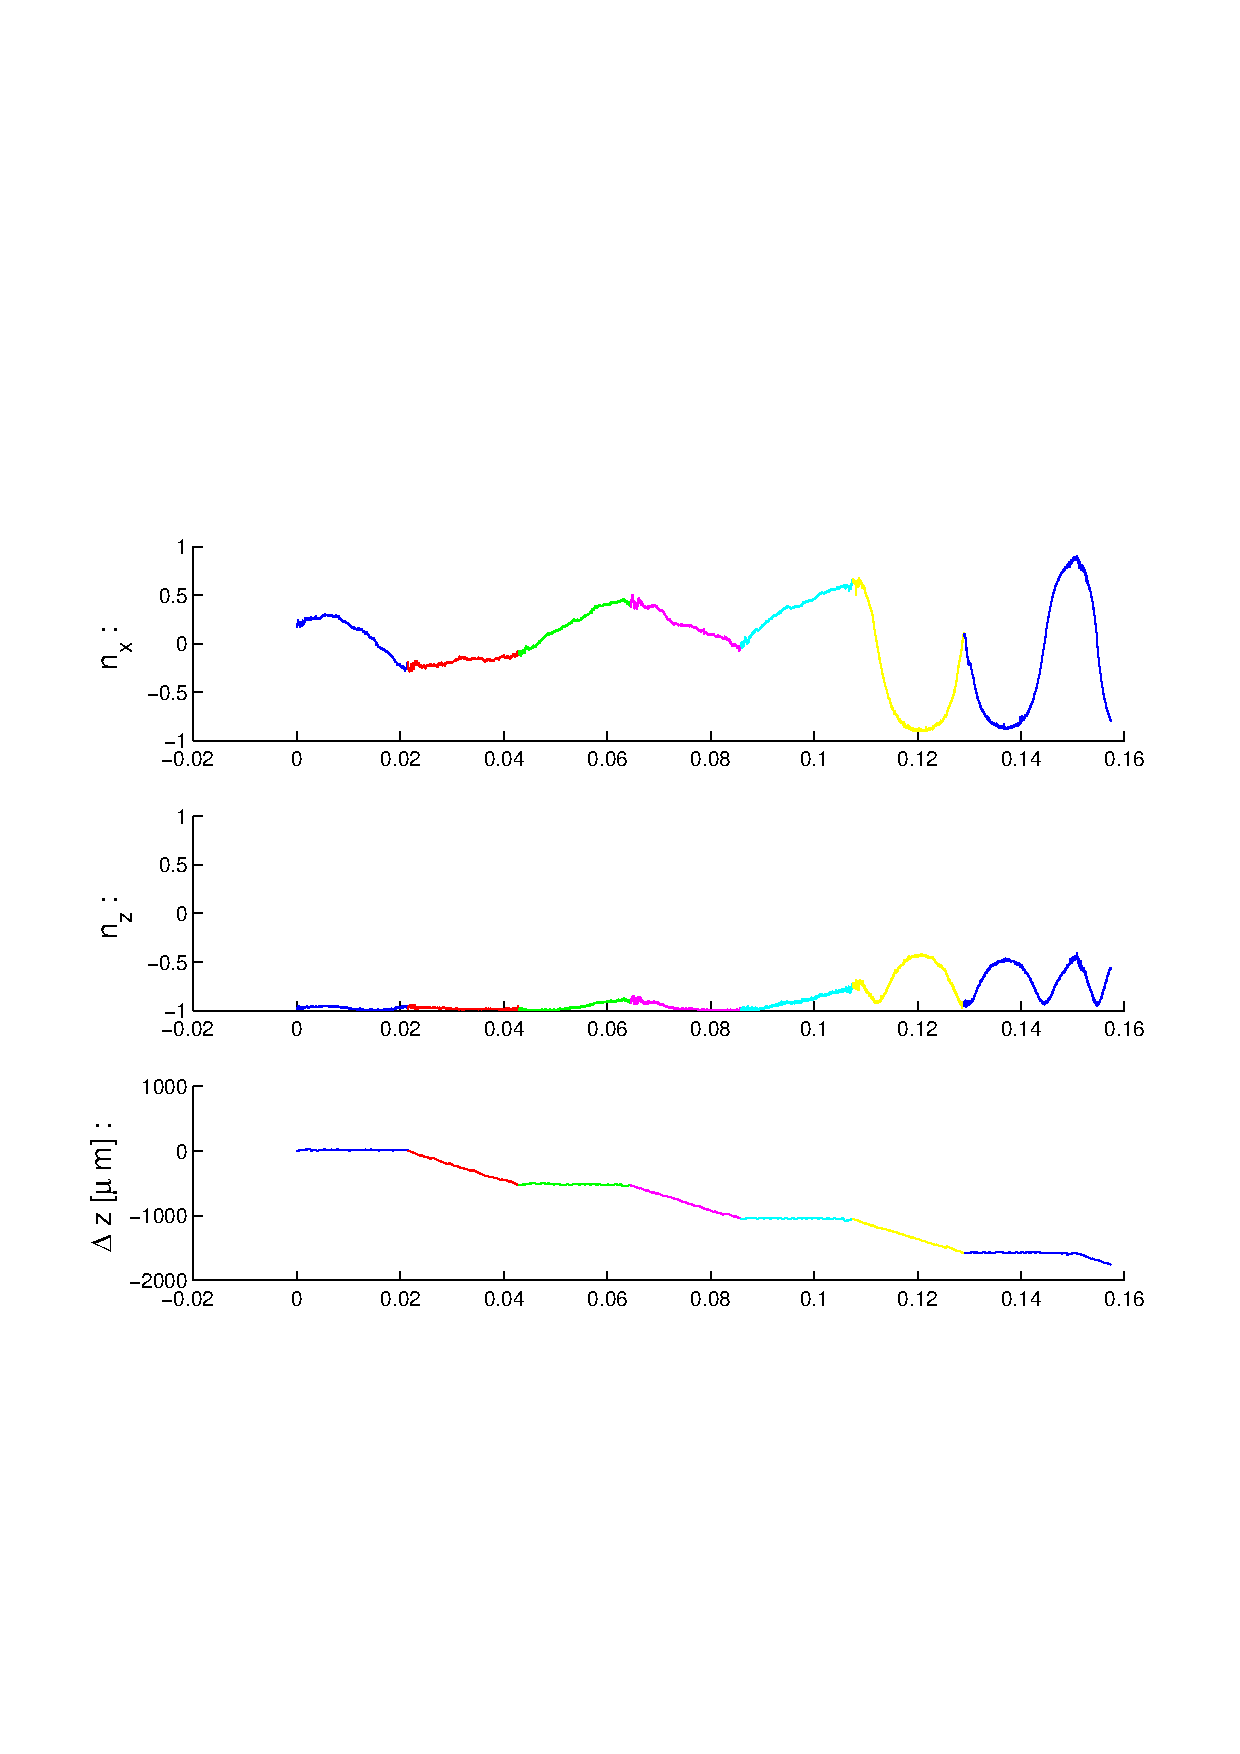
\includegraphics[width=0.8\textwidth]{Images/Particle 2/Particle2.pdf}

\end{figure}

\begin{figure}[ H]

\centering

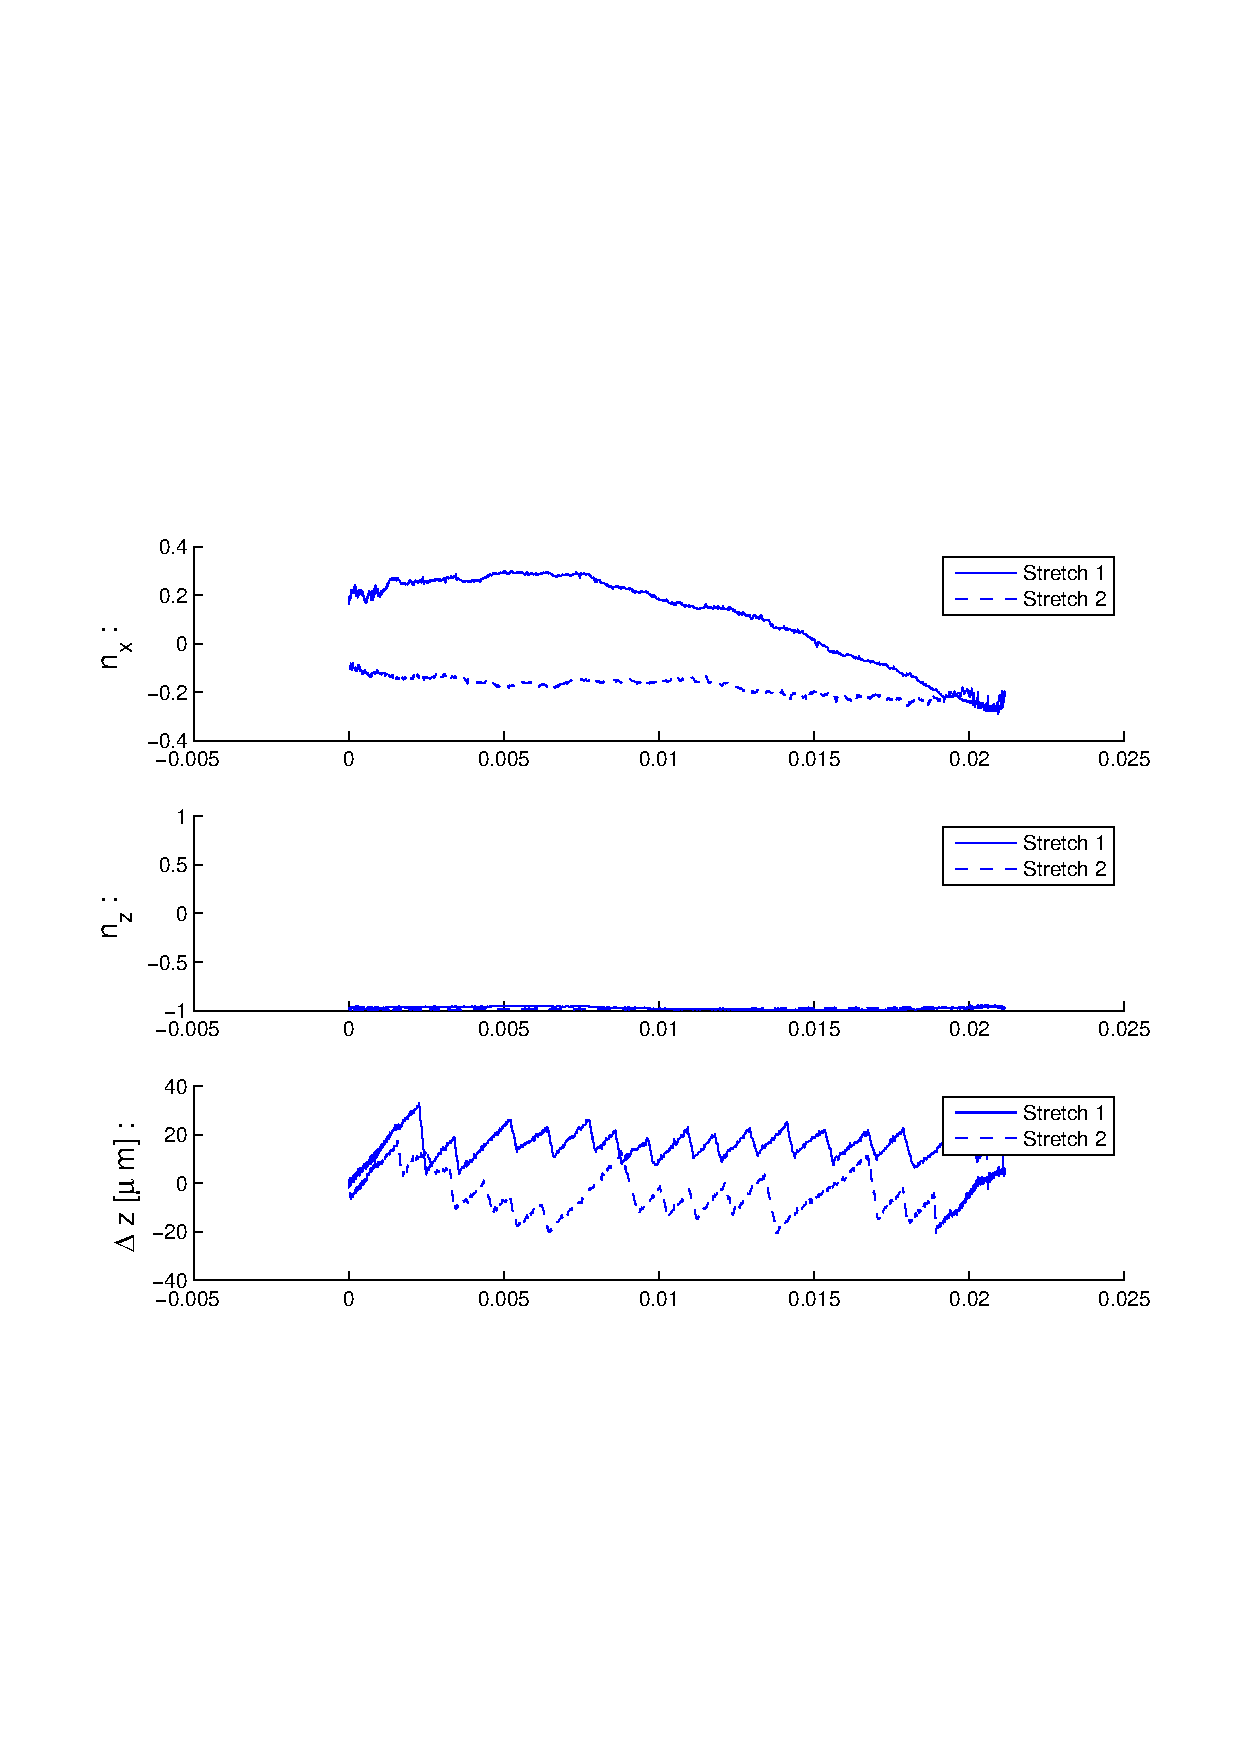
\includegraphics[width=0.8\textwidth]{Images/Particle 2/Stretch1.pdf}

\end{figure}

\begin{figure}[ H]

\centering

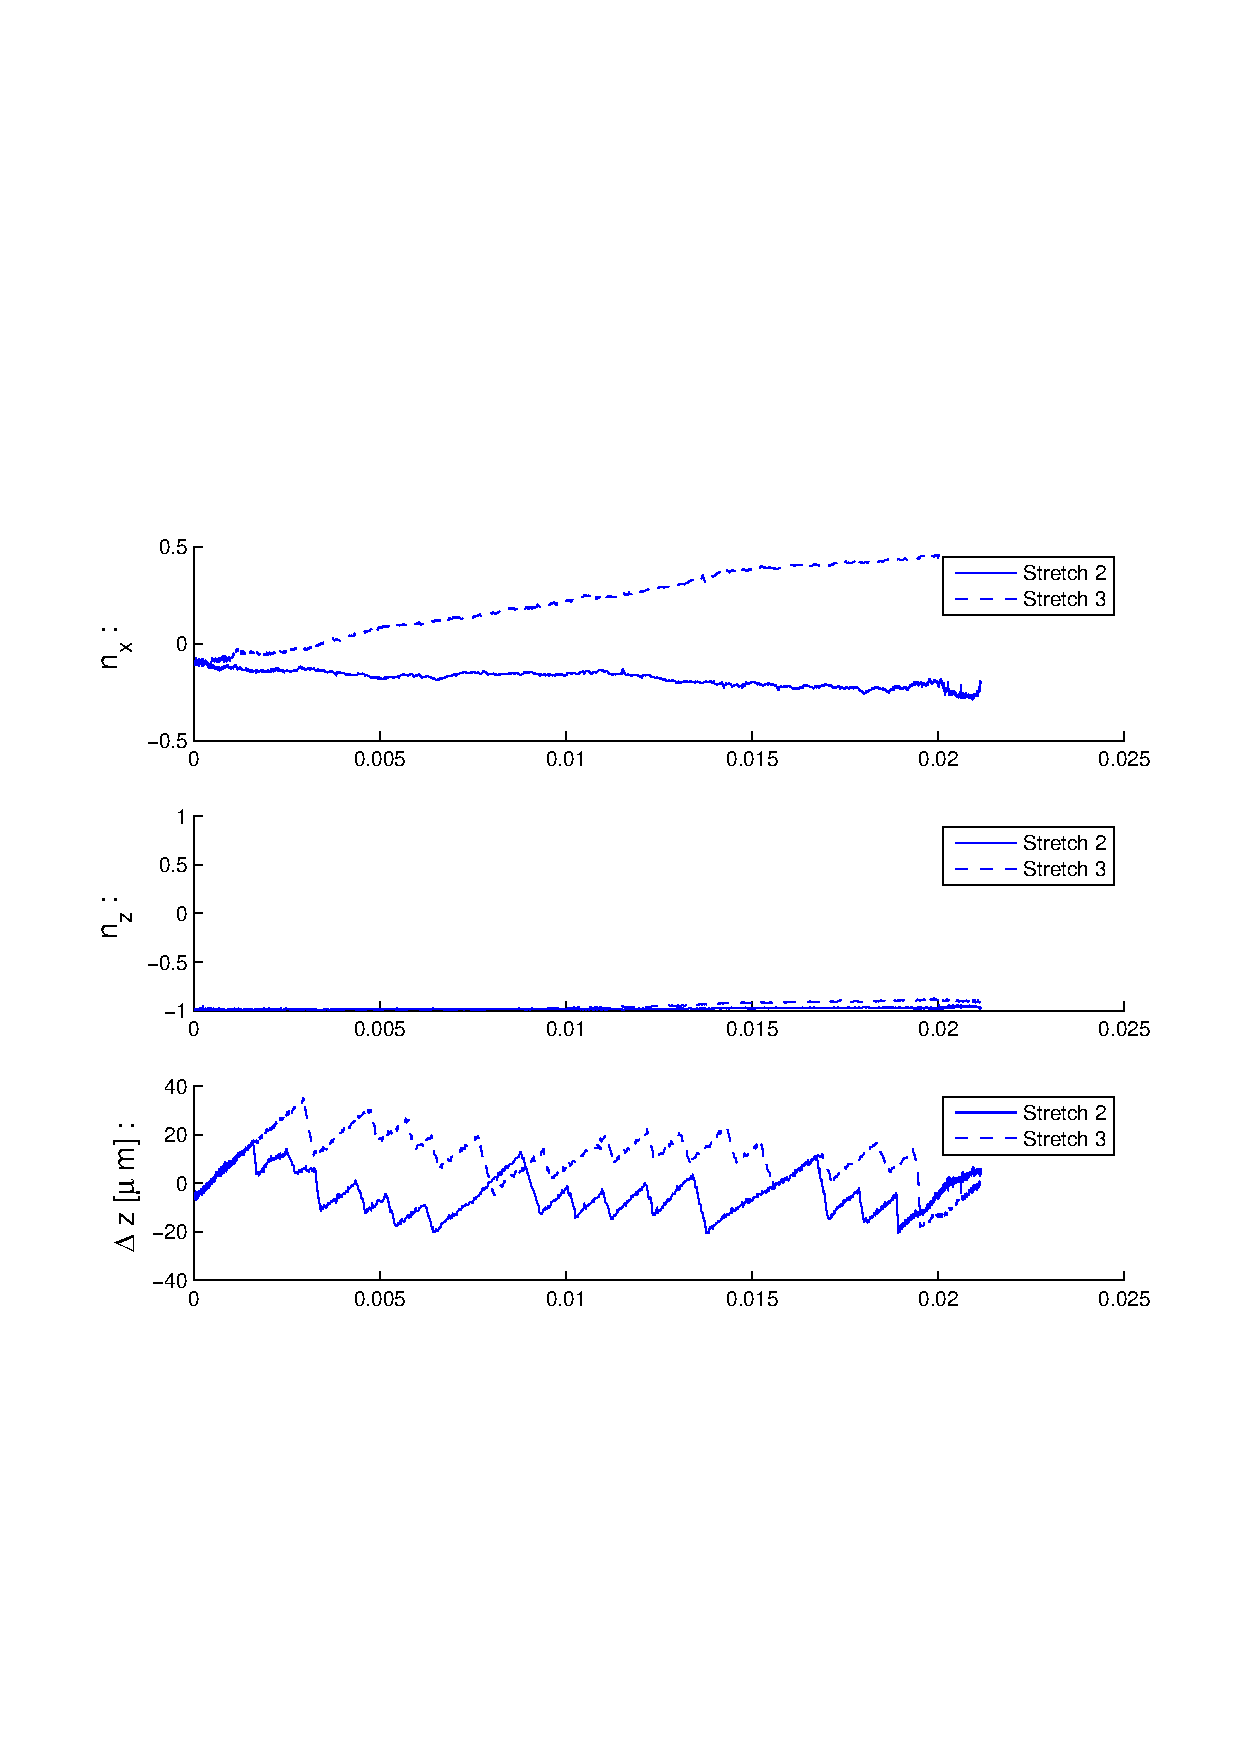
\includegraphics[width=0.8\textwidth]{Images/Particle 2/Stretch2.pdf}

\end{figure}

\begin{figure}[ H]

\centering

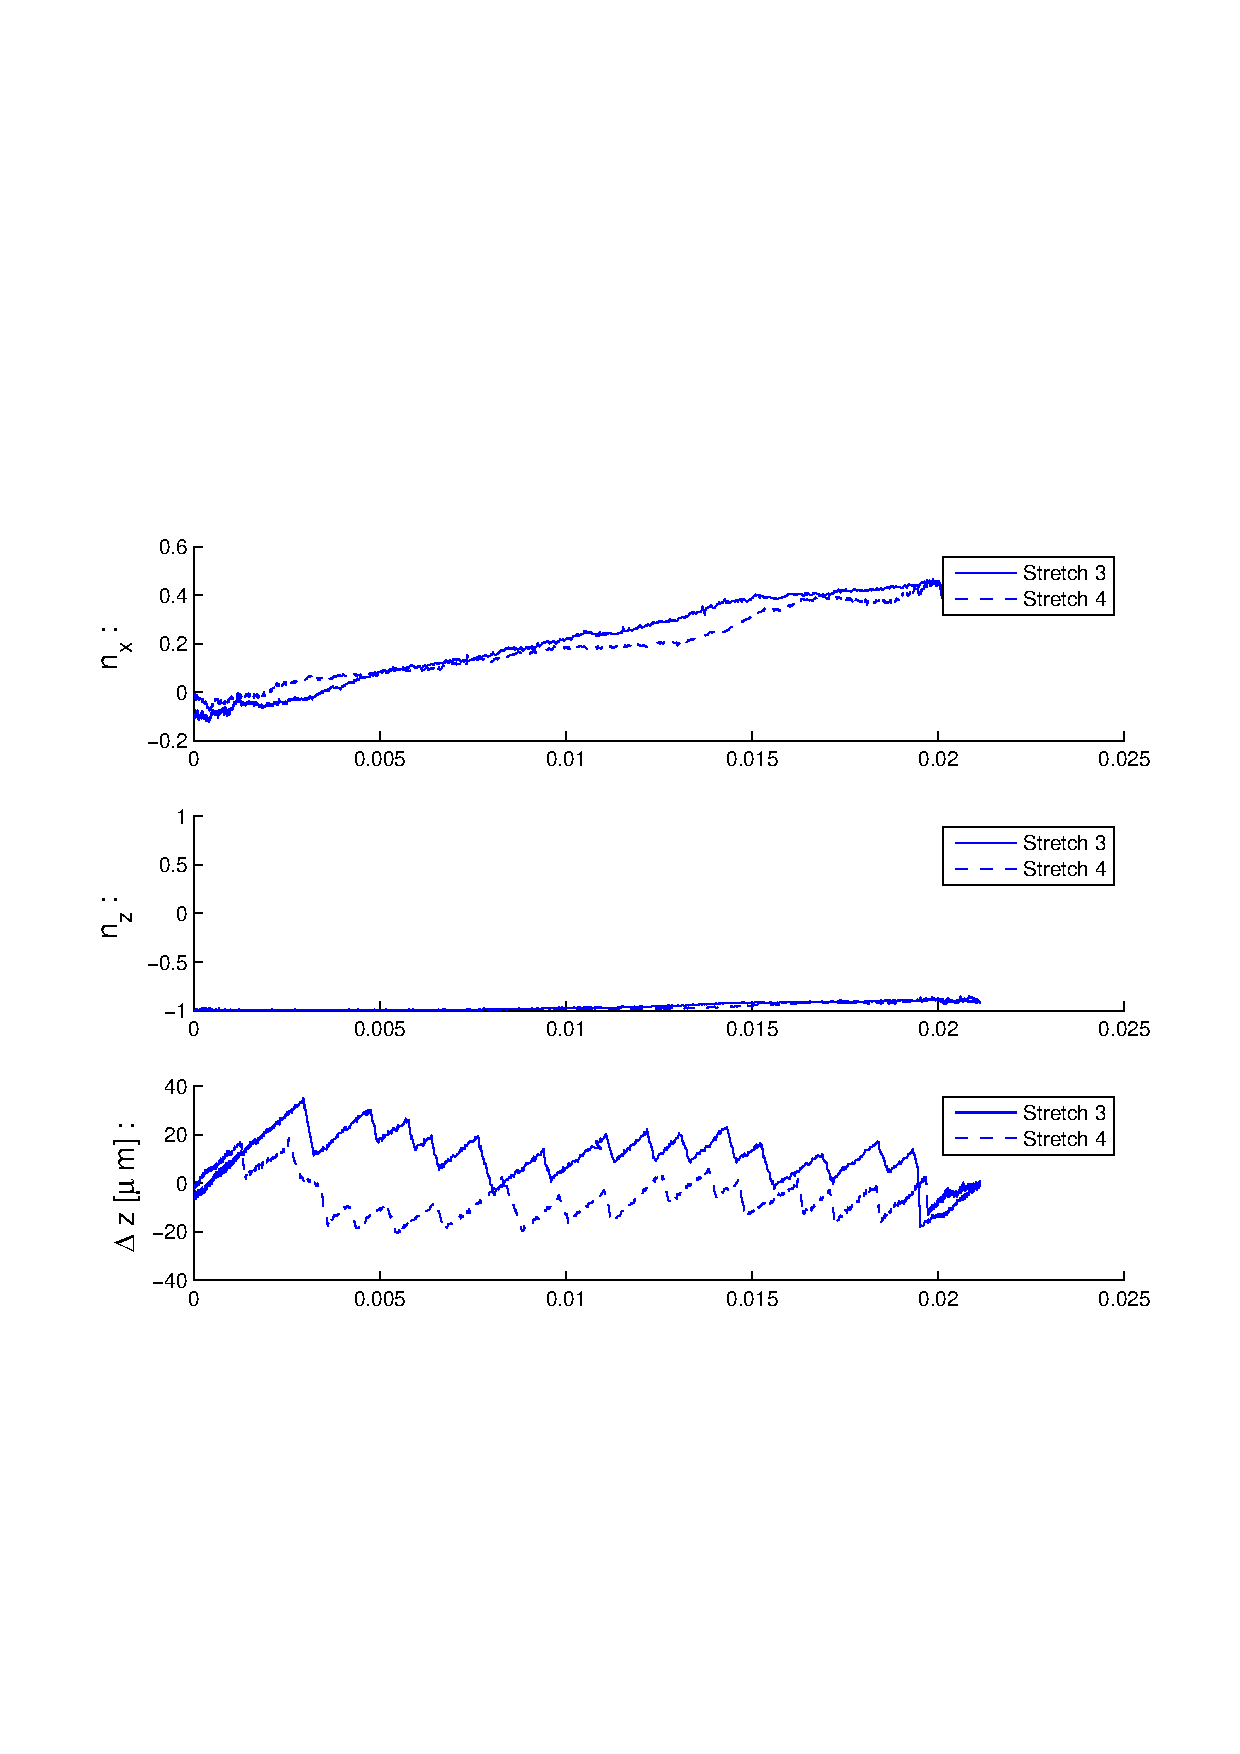
\includegraphics[width=0.8\textwidth]{Images/Particle 2/Stretch3.pdf}

\end{figure}

\begin{figure}[ H]

\centering

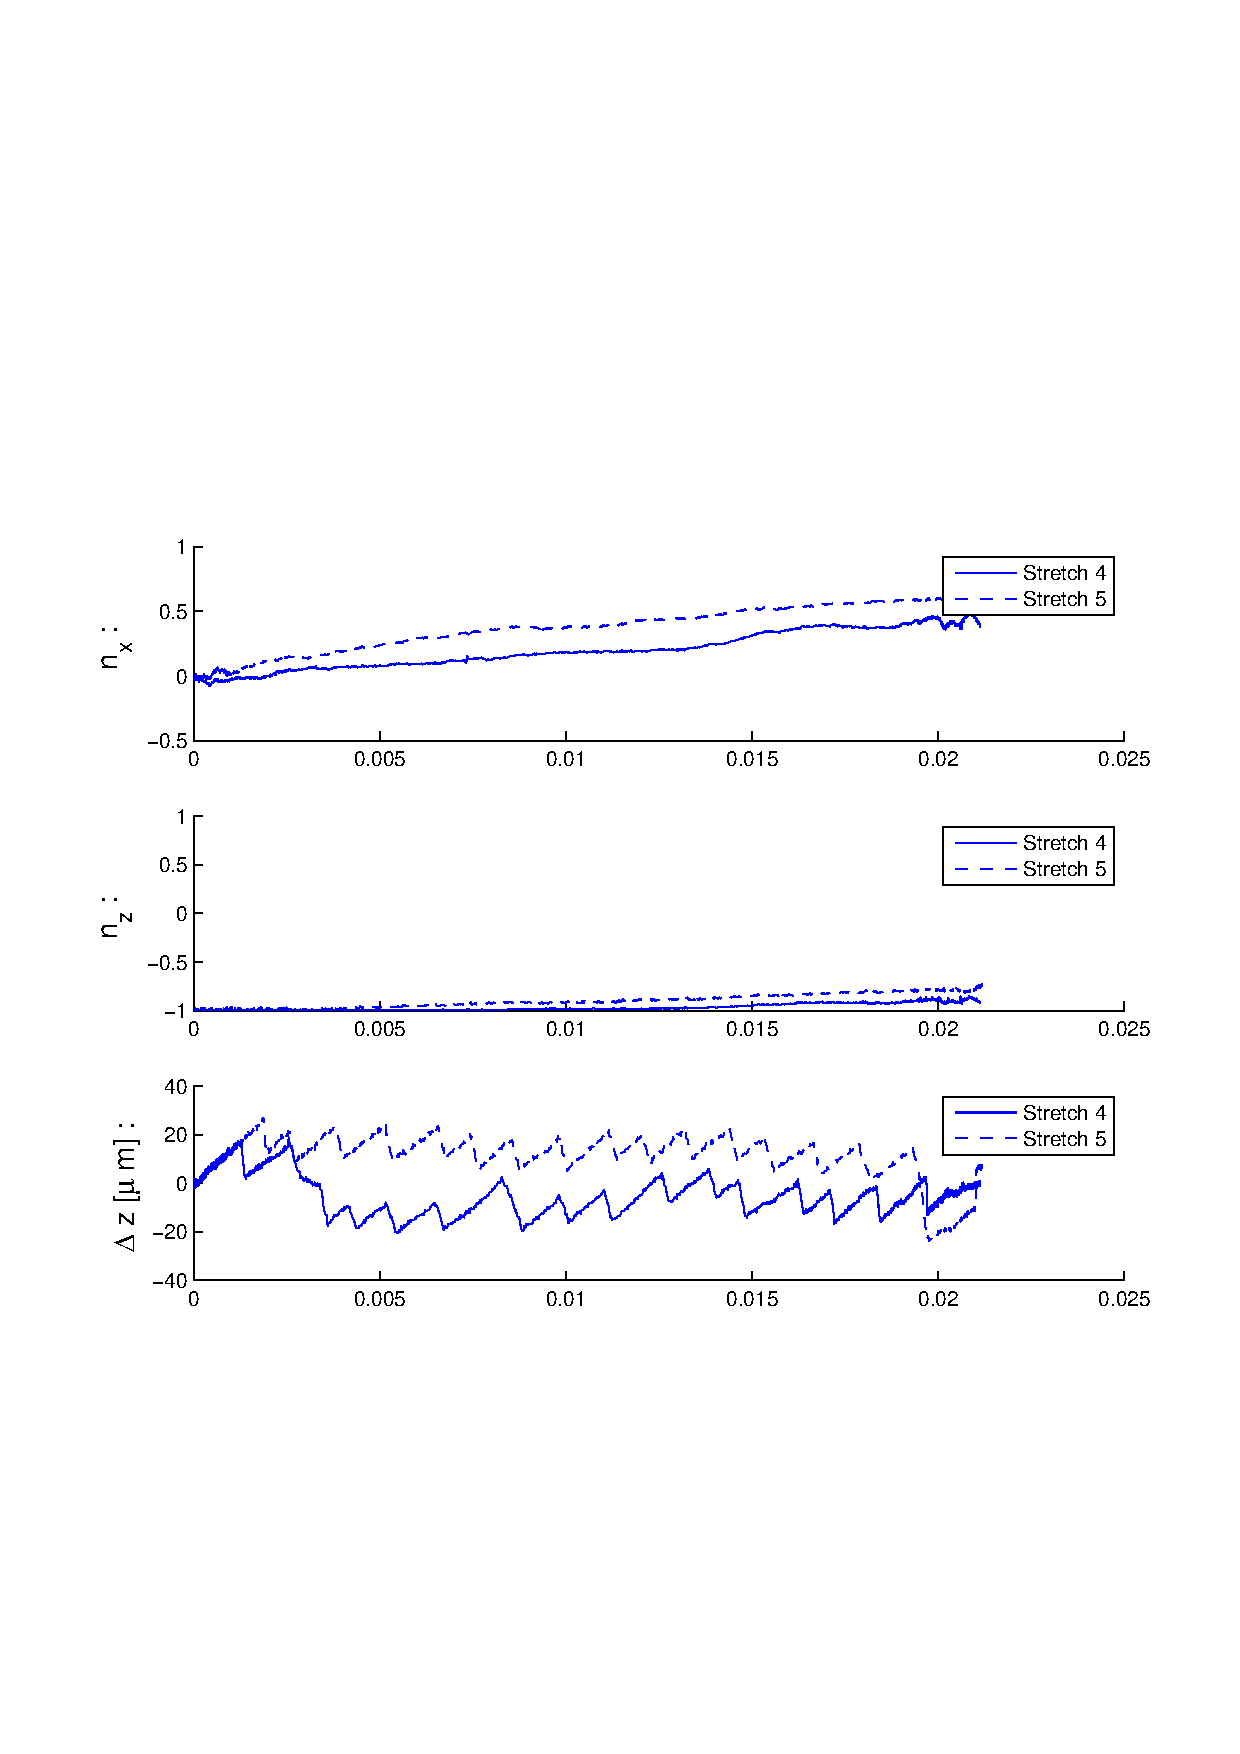
\includegraphics[width=0.8\textwidth]{Images/Particle 2/Stretch4.pdf}

\end{figure}

\begin{figure}[ H]

\centering

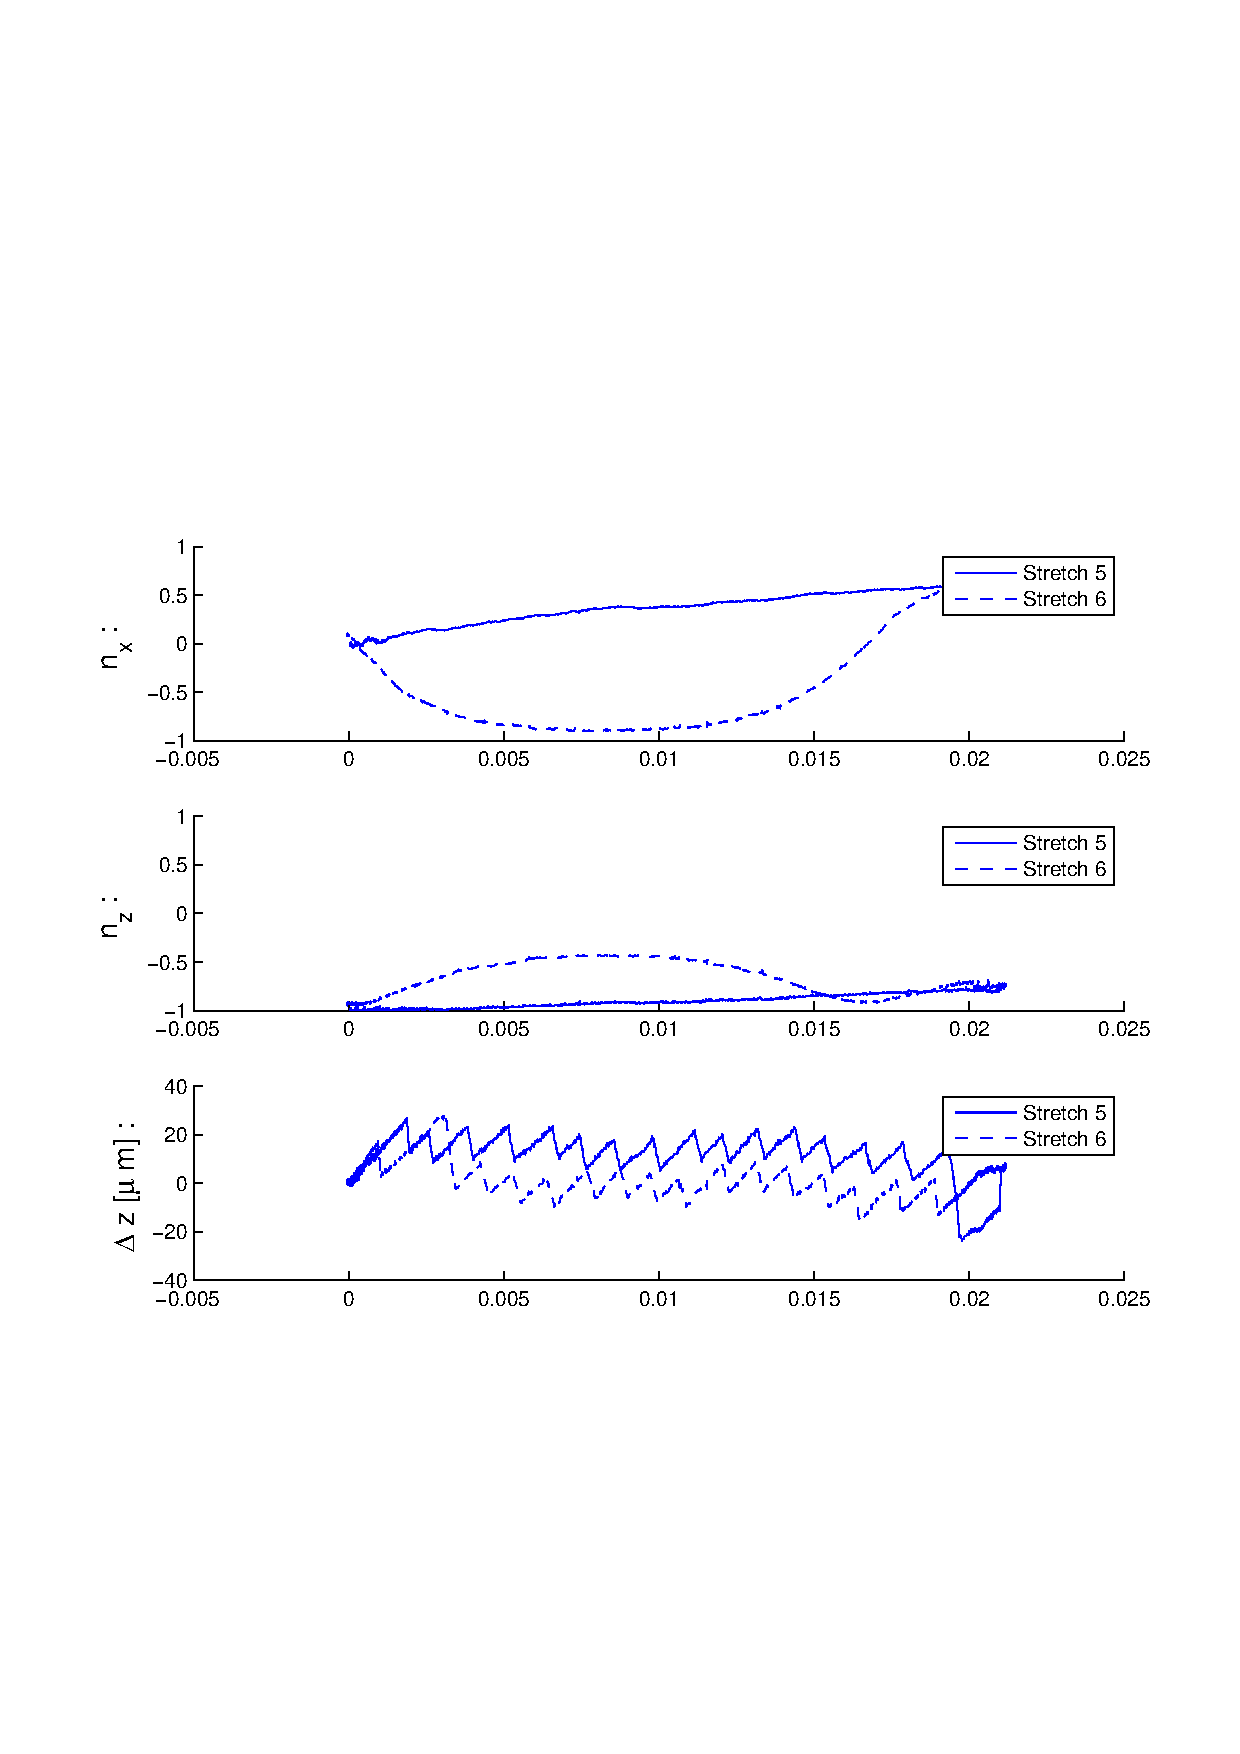
\includegraphics[width=0.8\textwidth]{Images/Particle 2/Stretch5.pdf}

\end{figure}

\begin{figure}[ H]

\centering

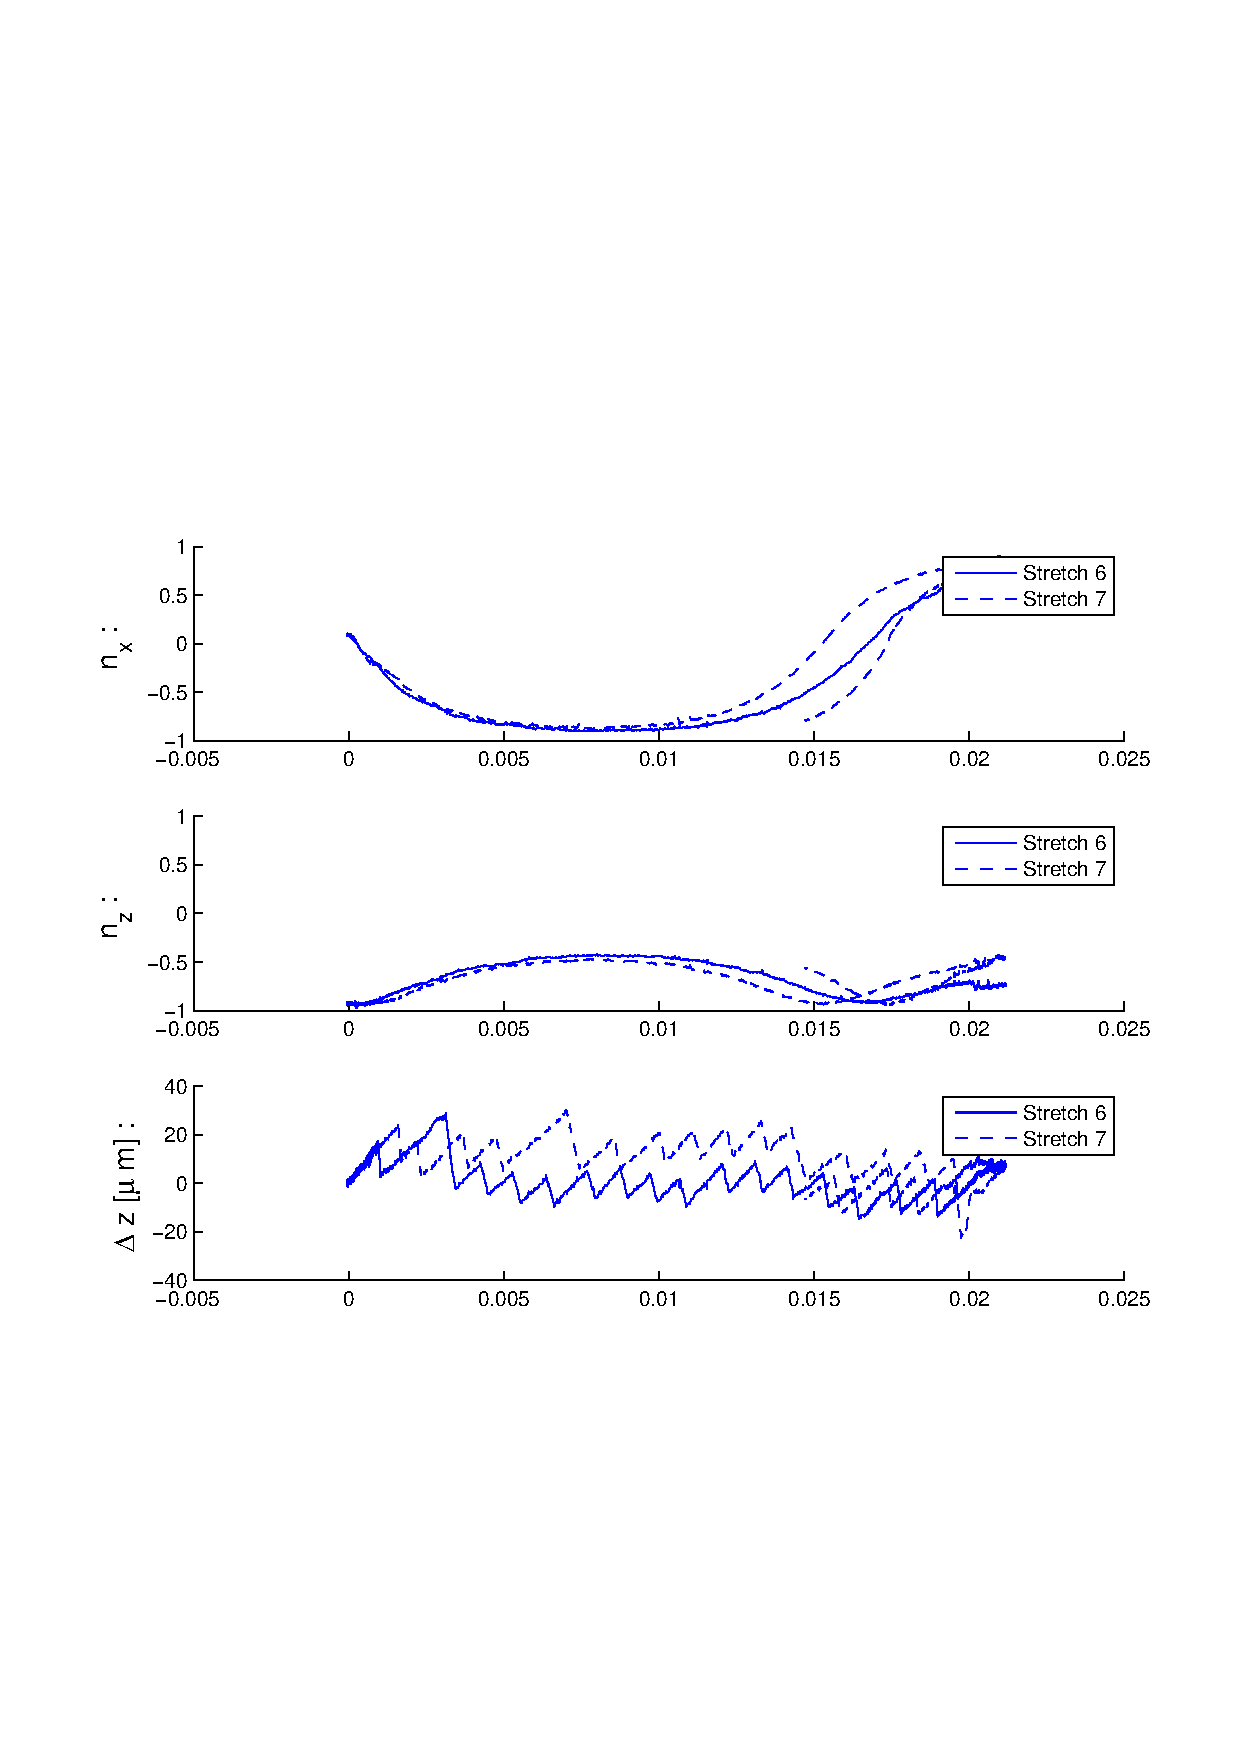
\includegraphics[width=0.8\textwidth]{Images/Particle 2/Stretch6.pdf}

\end{figure}


\subsection{Particle 7}

\begin{figure}[ H]

\caption{Particle 7: $ \lambda: 27.4694$Depth: 20 out of $200 \mu $ m}

\centering

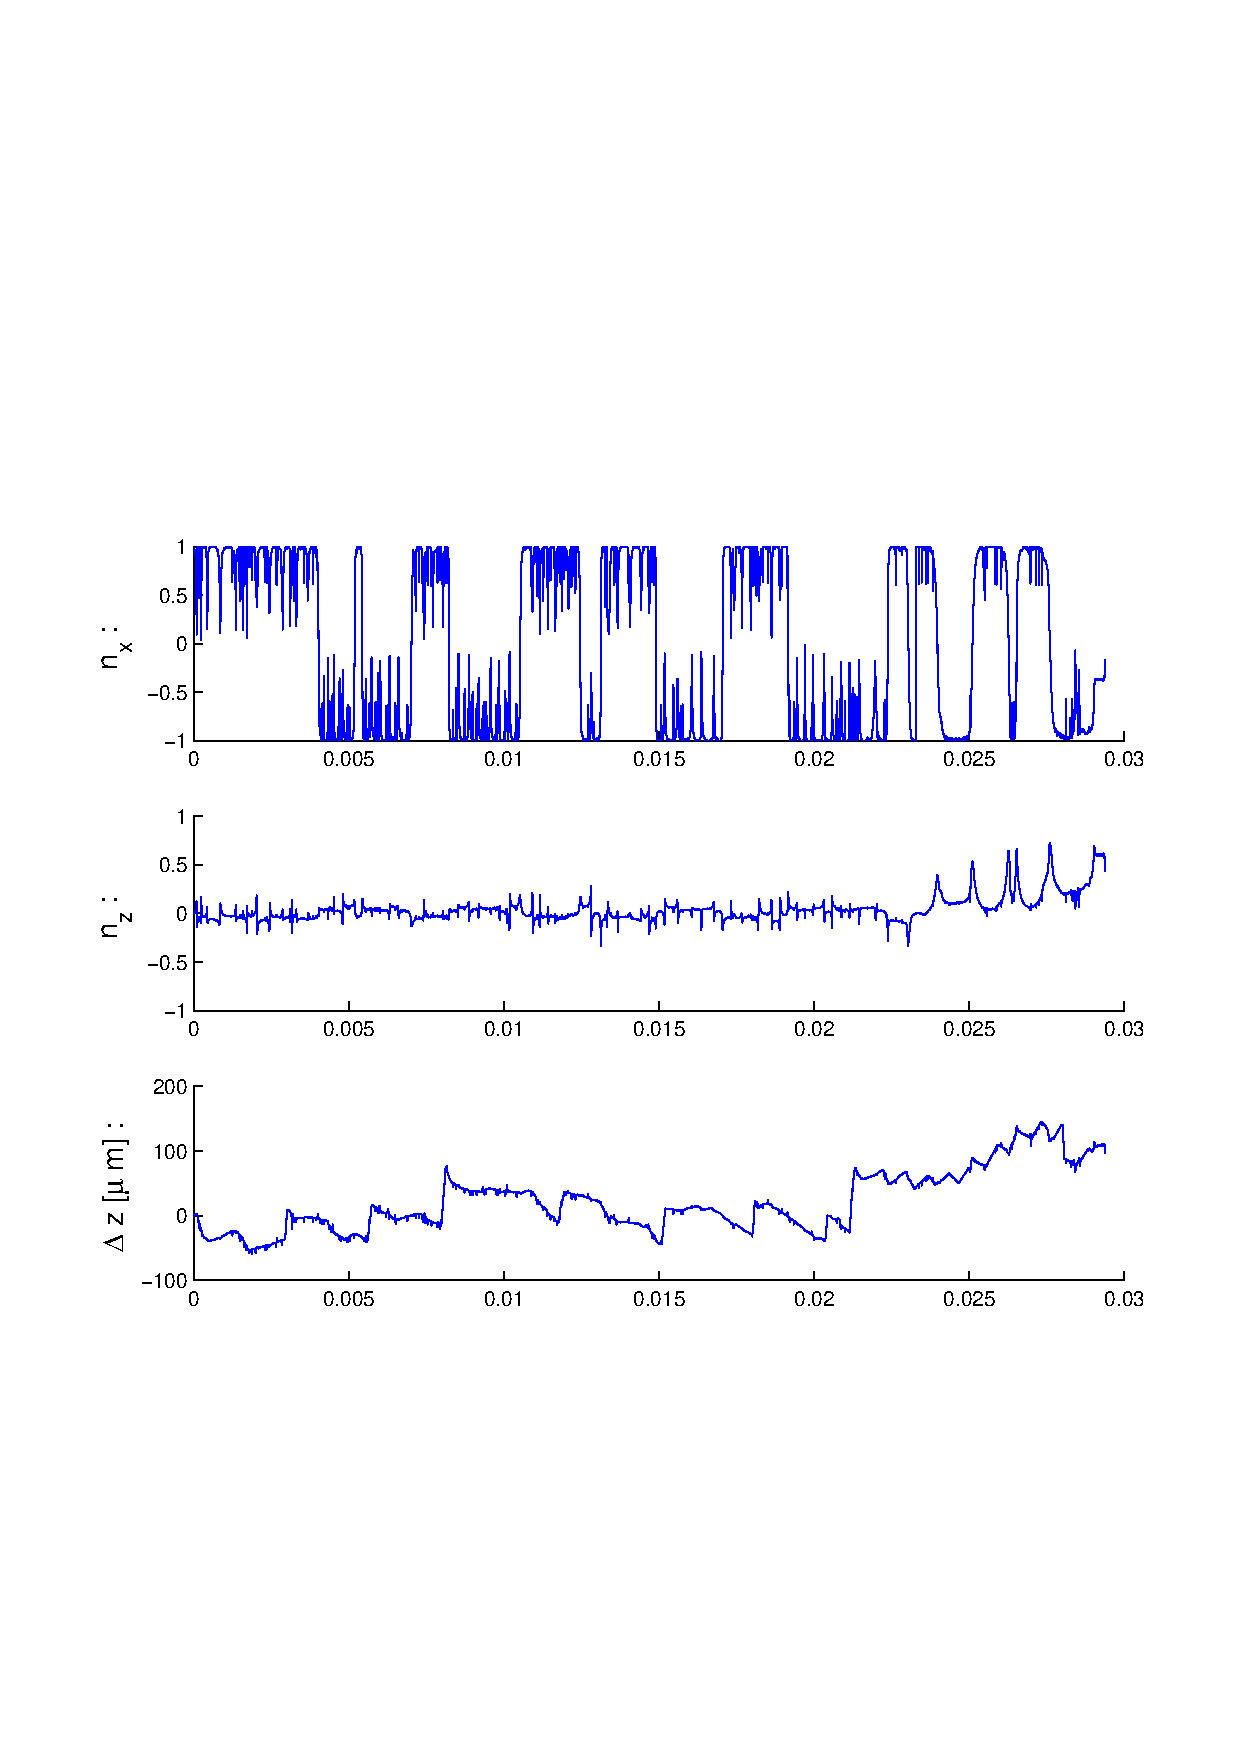
\includegraphics[width=0.8\textwidth]{Images/Particle 7/Particle7.pdf}

\end{figure}


\subsection{Particle 18}

\begin{figure}[ H]

\caption{Particle 18: Unclear. There are several possible interactions around 6 minutes but neither is all too clear. Also the second turn is overall quite jumpy$ \lambda: 14.3568$Depth: 20 out of $200 \mu $ m}

\centering

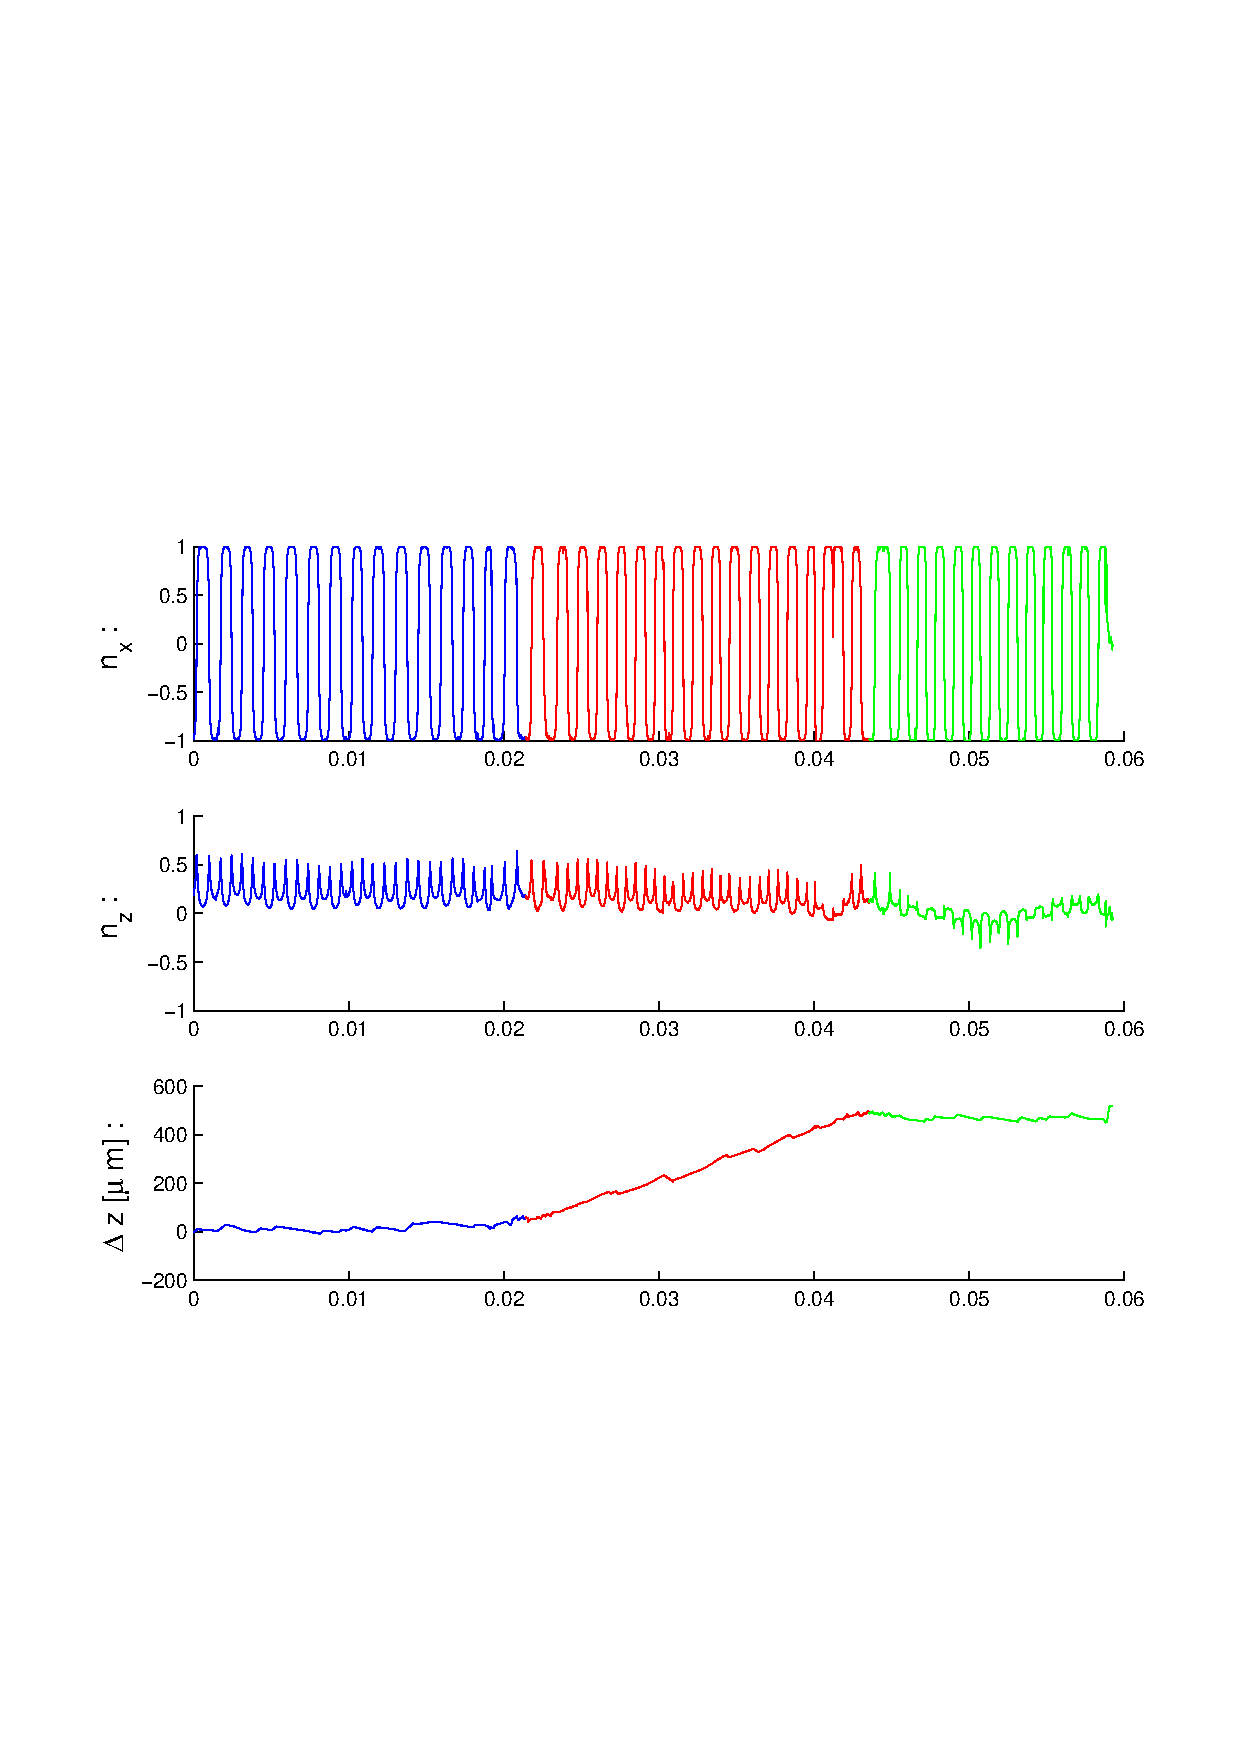
\includegraphics[width=0.8\textwidth]{Images/Particle 18/Particle18.pdf}

\end{figure}

\begin{figure}[ H]

\centering

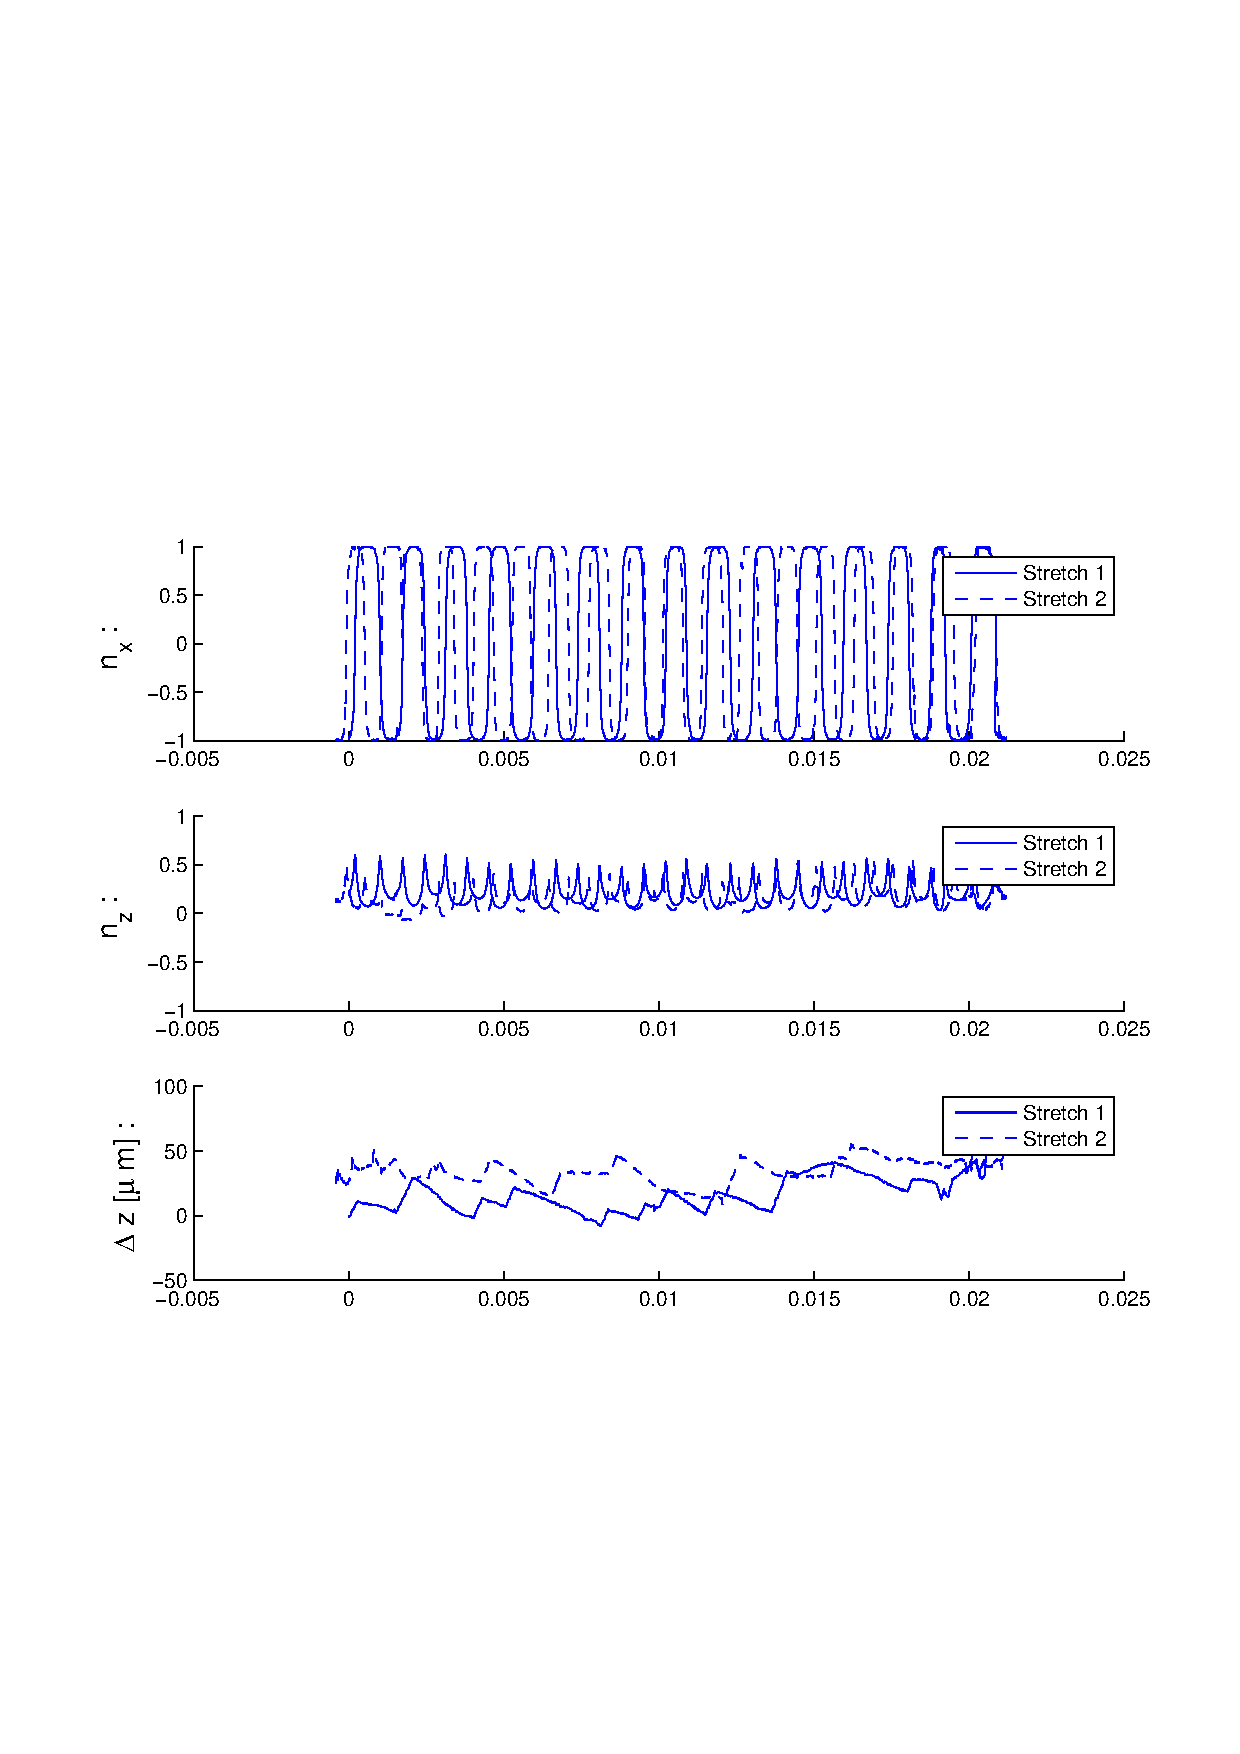
\includegraphics[width=0.8\textwidth]{Images/Particle 18/Stretch1.pdf}

\end{figure}

\begin{figure}[ H]

\centering

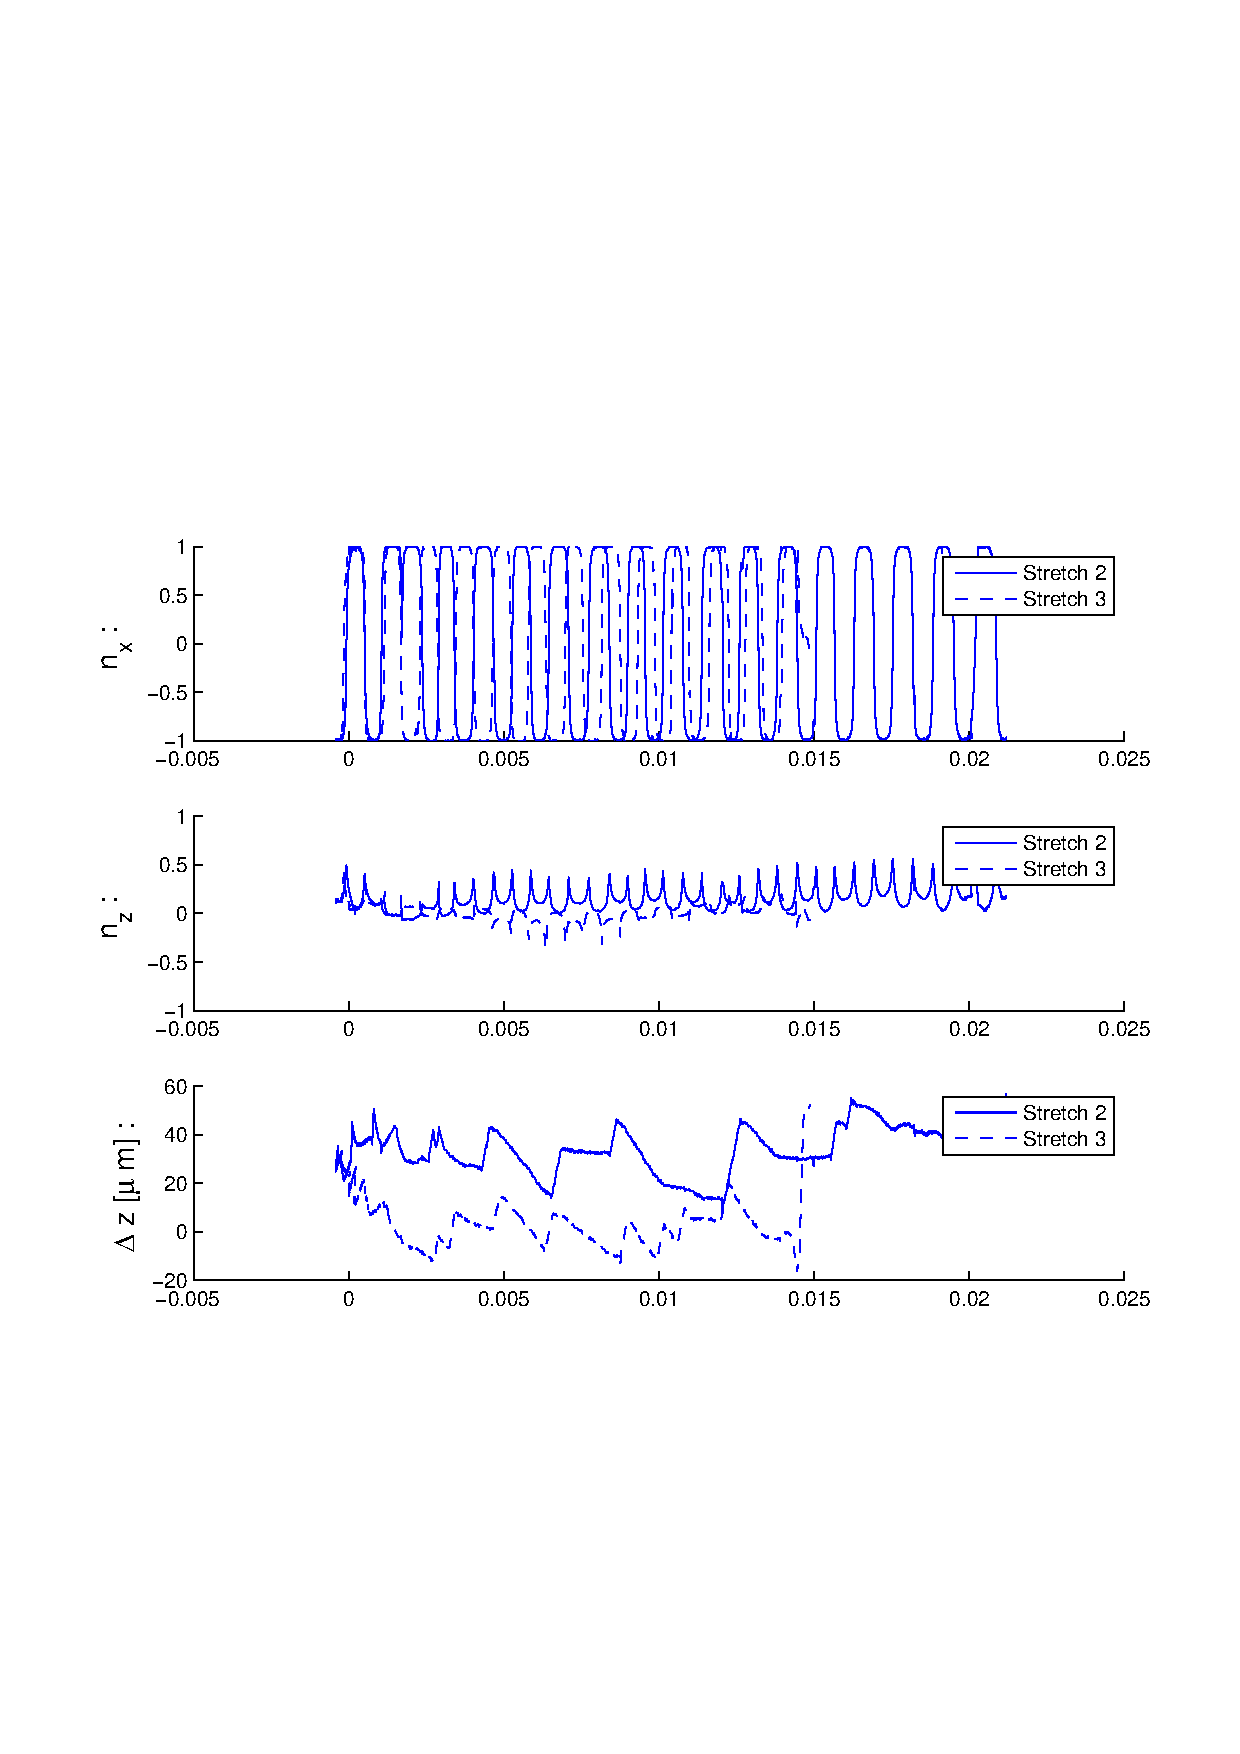
\includegraphics[width=0.8\textwidth]{Images/Particle 18/Stretch2.pdf}

\end{figure}


\subsection{Particle 19}

\begin{figure}[ H]

\caption{Particle 19: At around 0:50 there is an uneven vertical flow "surging" the particle down. $ \lambda: 13.795$Depth: 120 out of $200 \mu $ m}

\centering

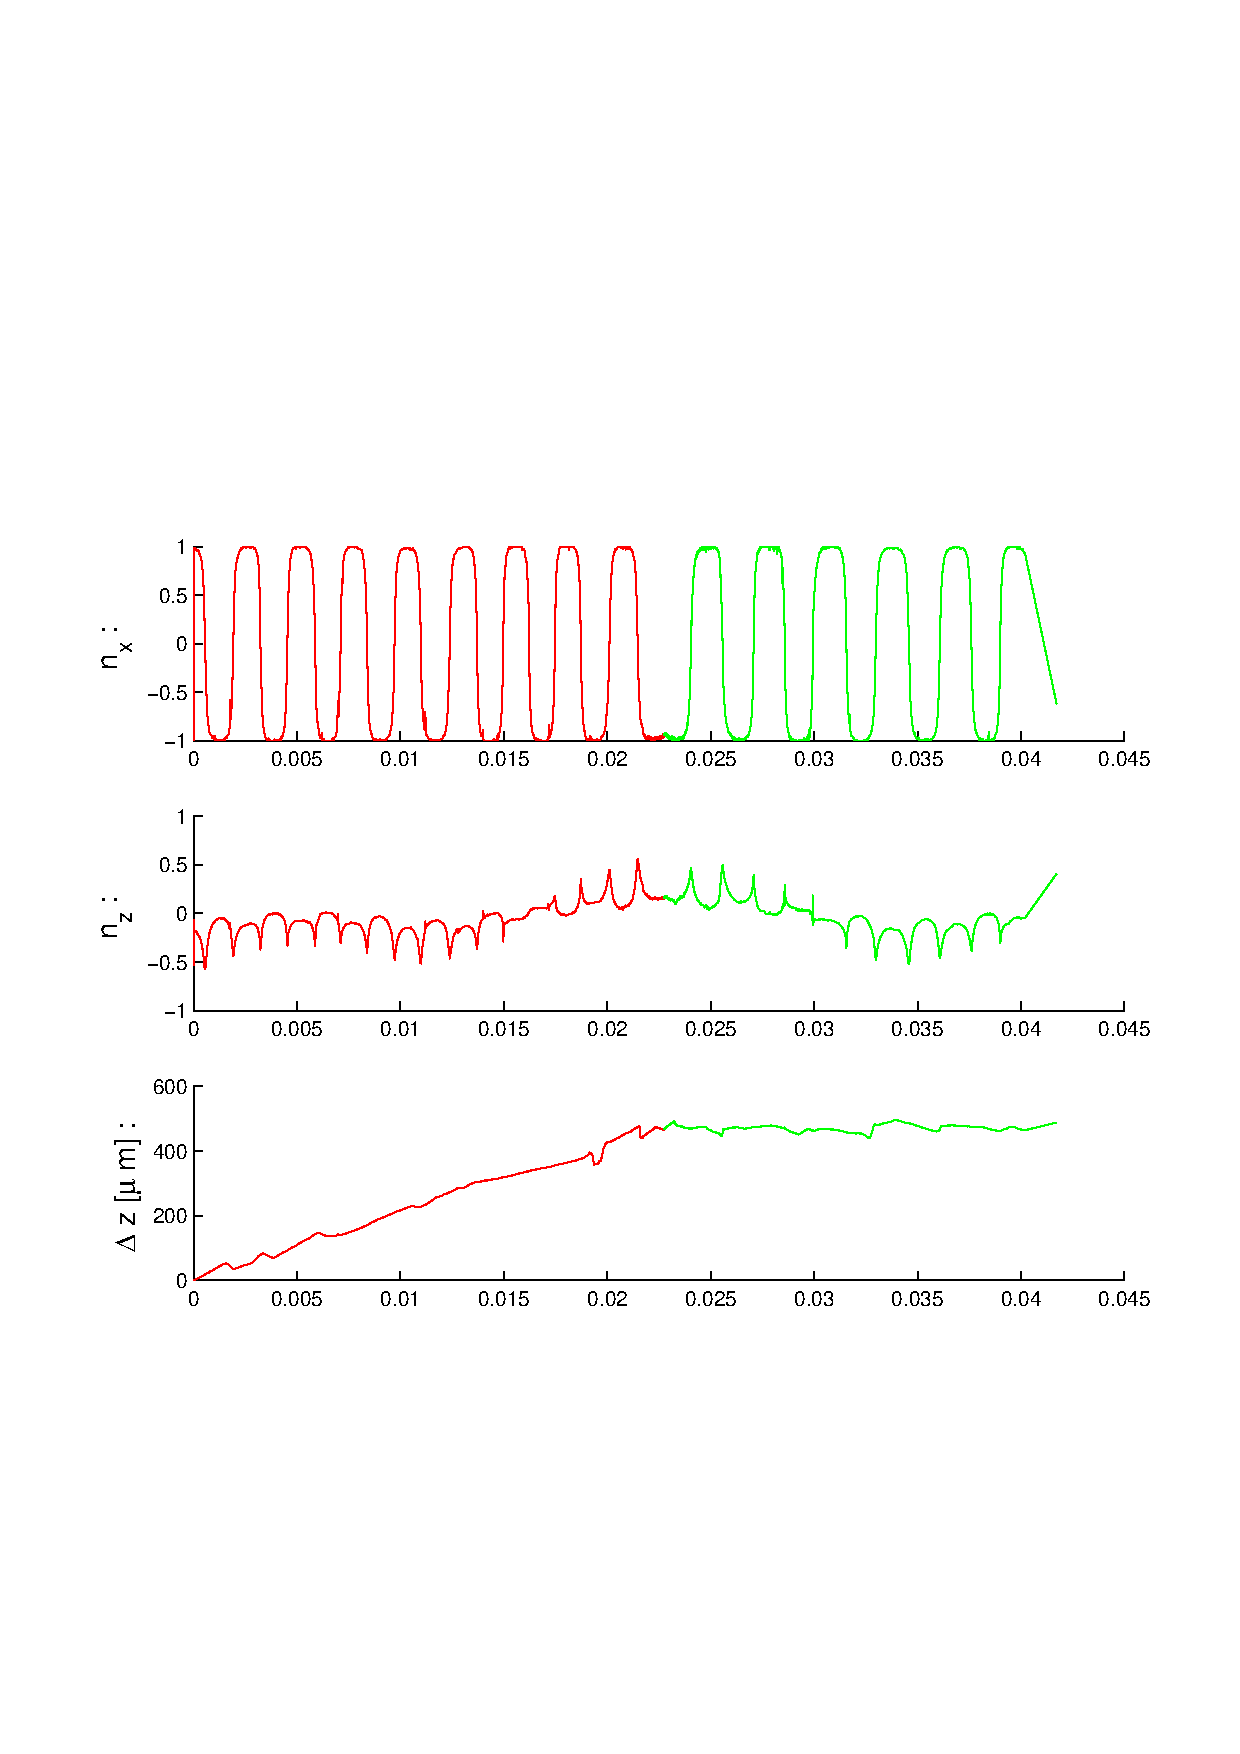
\includegraphics[width=0.8\textwidth]{Images/Particle 19/Particle19.pdf}

\end{figure}

\begin{figure}[ H]

\centering

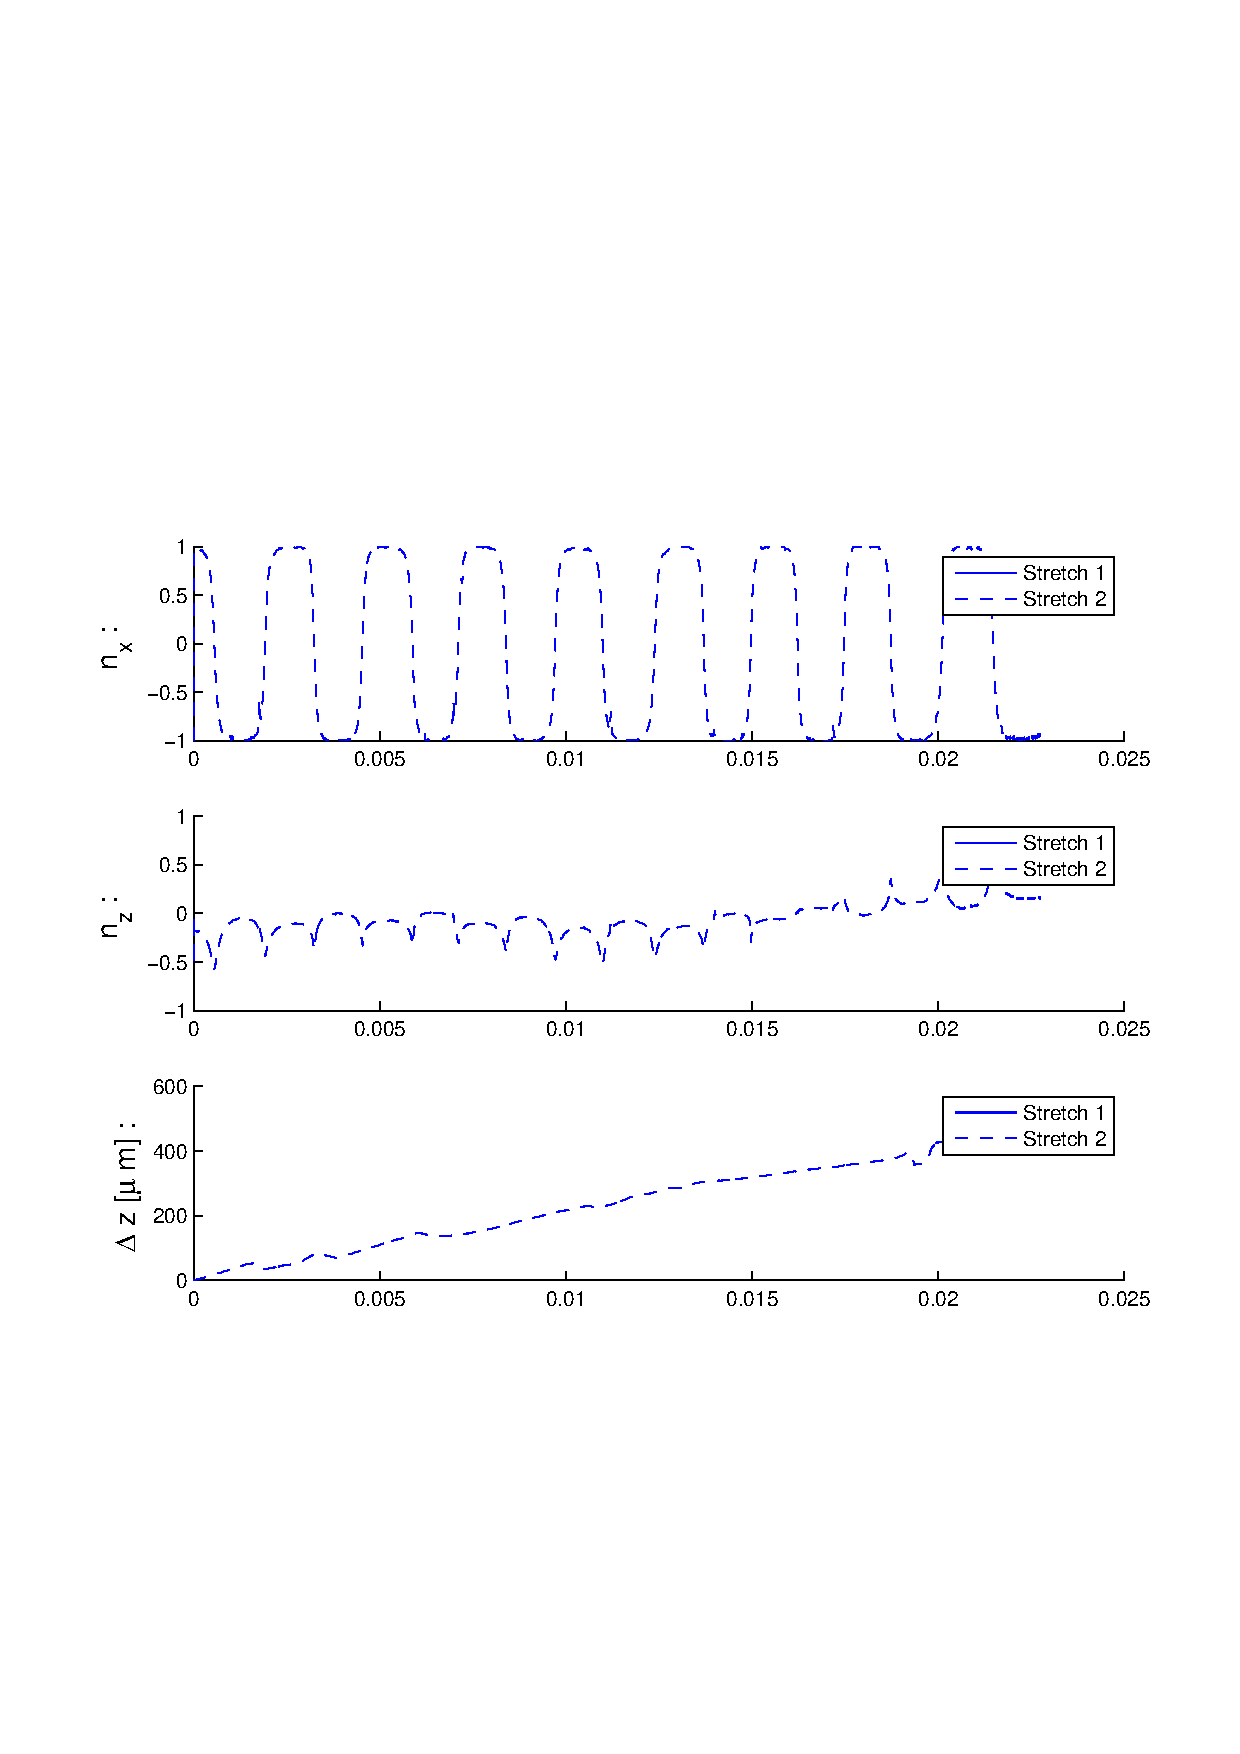
\includegraphics[width=0.8\textwidth]{Images/Particle 19/Stretch1.pdf}

\end{figure}

\begin{figure}[ H]

\centering

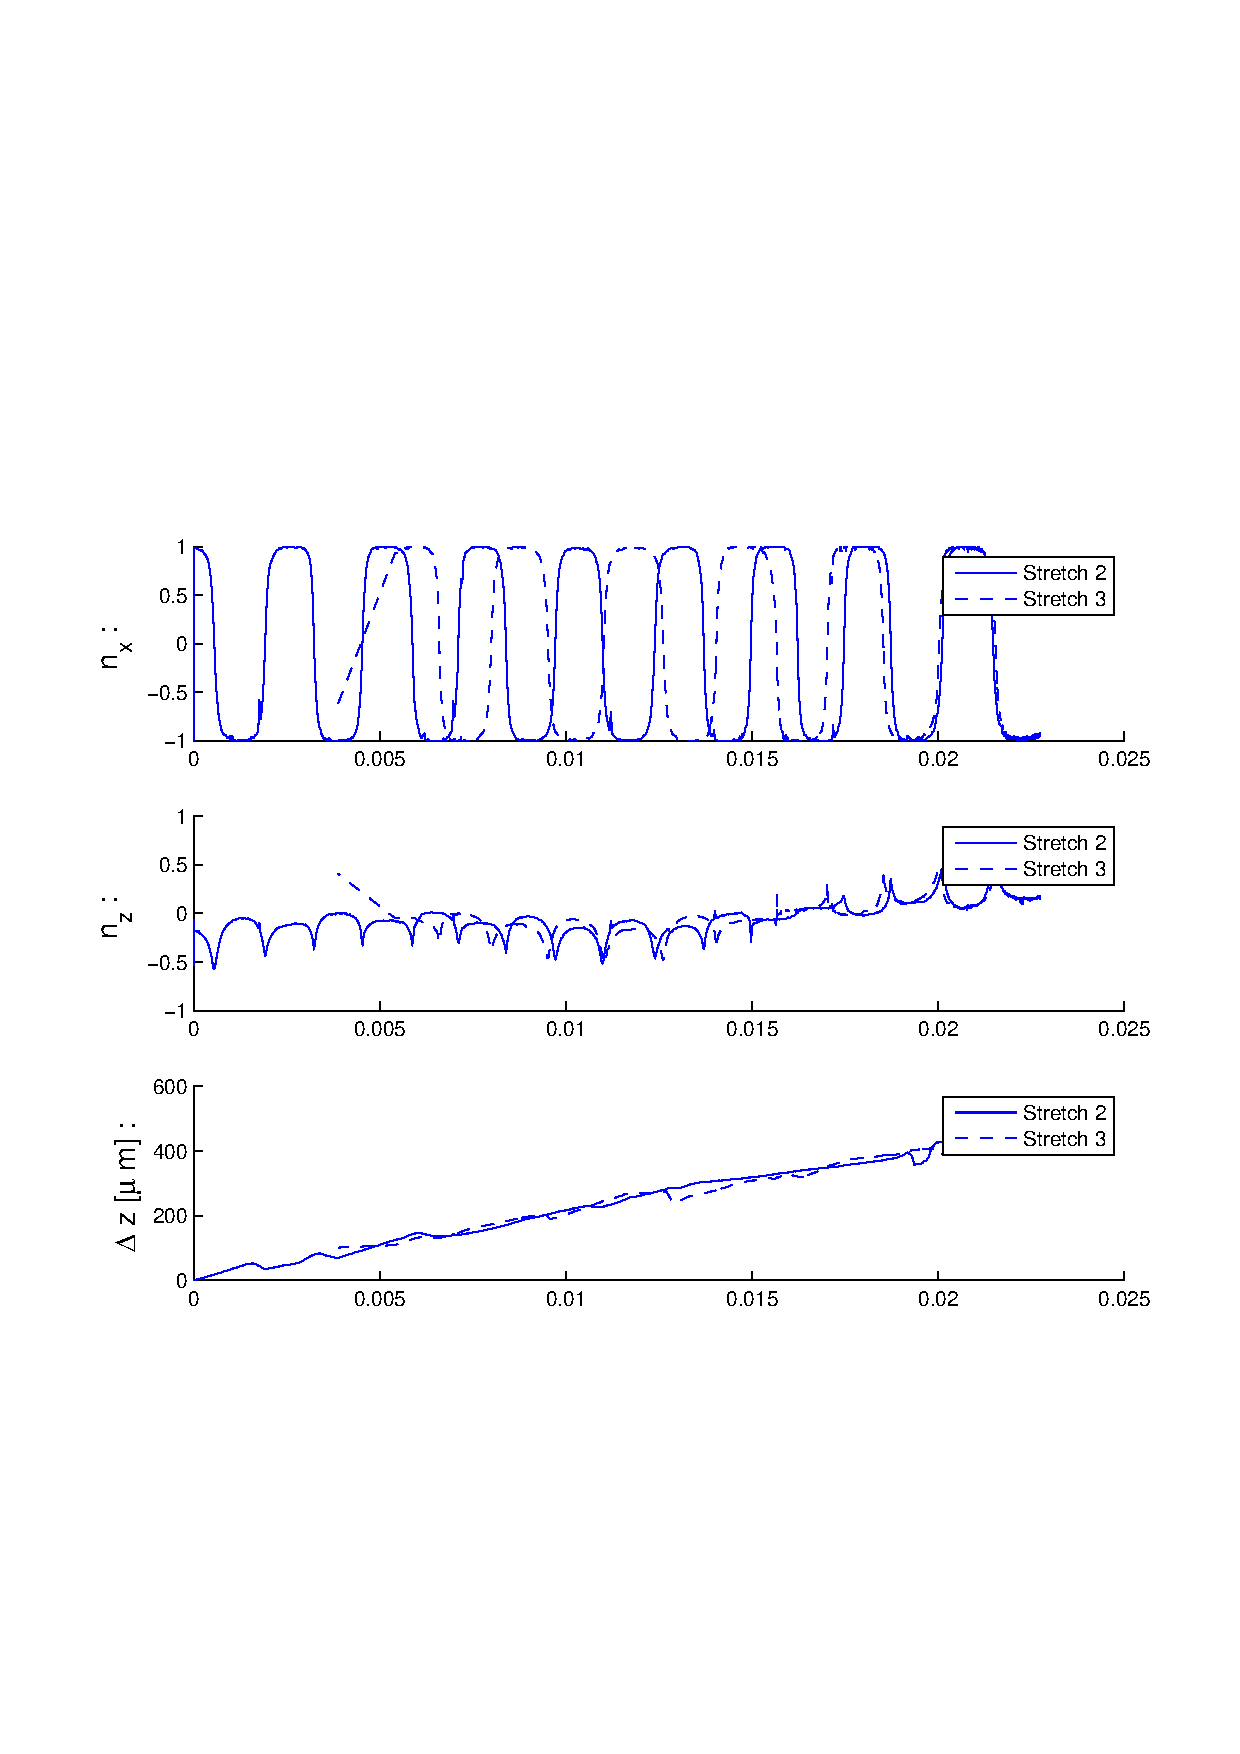
\includegraphics[width=0.8\textwidth]{Images/Particle 19/Stretch2.pdf}

\end{figure}



 


\subsection{Particle 20}

\begin{figure}[ H]

\caption{Particle 20: At 5:22 collides with large "debris" on channel floor. $ \lambda: 13.5864$Depth: 150 out of $200 \mu $ m}

\centering

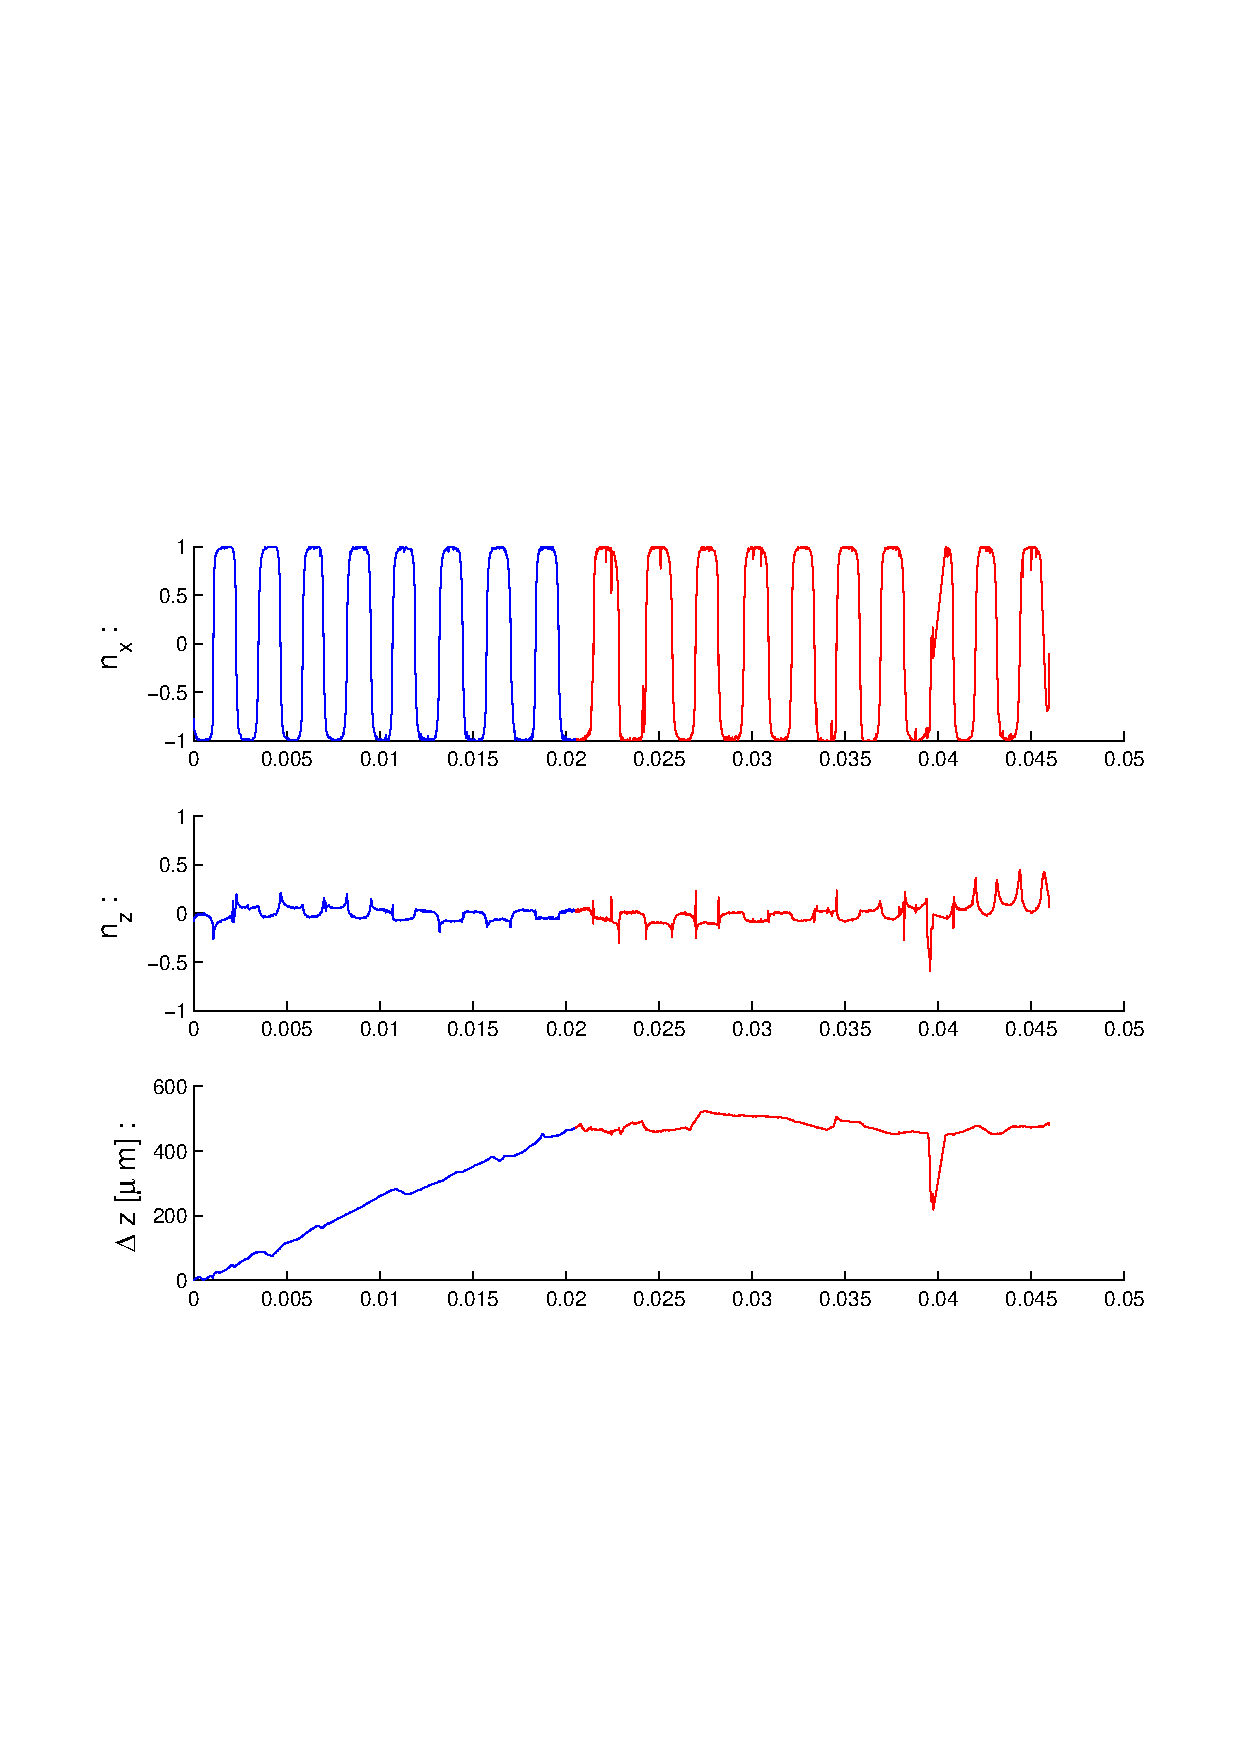
\includegraphics[width=0.8\textwidth]{Images/Particle 20/Particle20.pdf}

\end{figure}

\begin{figure}[ H]

\centering

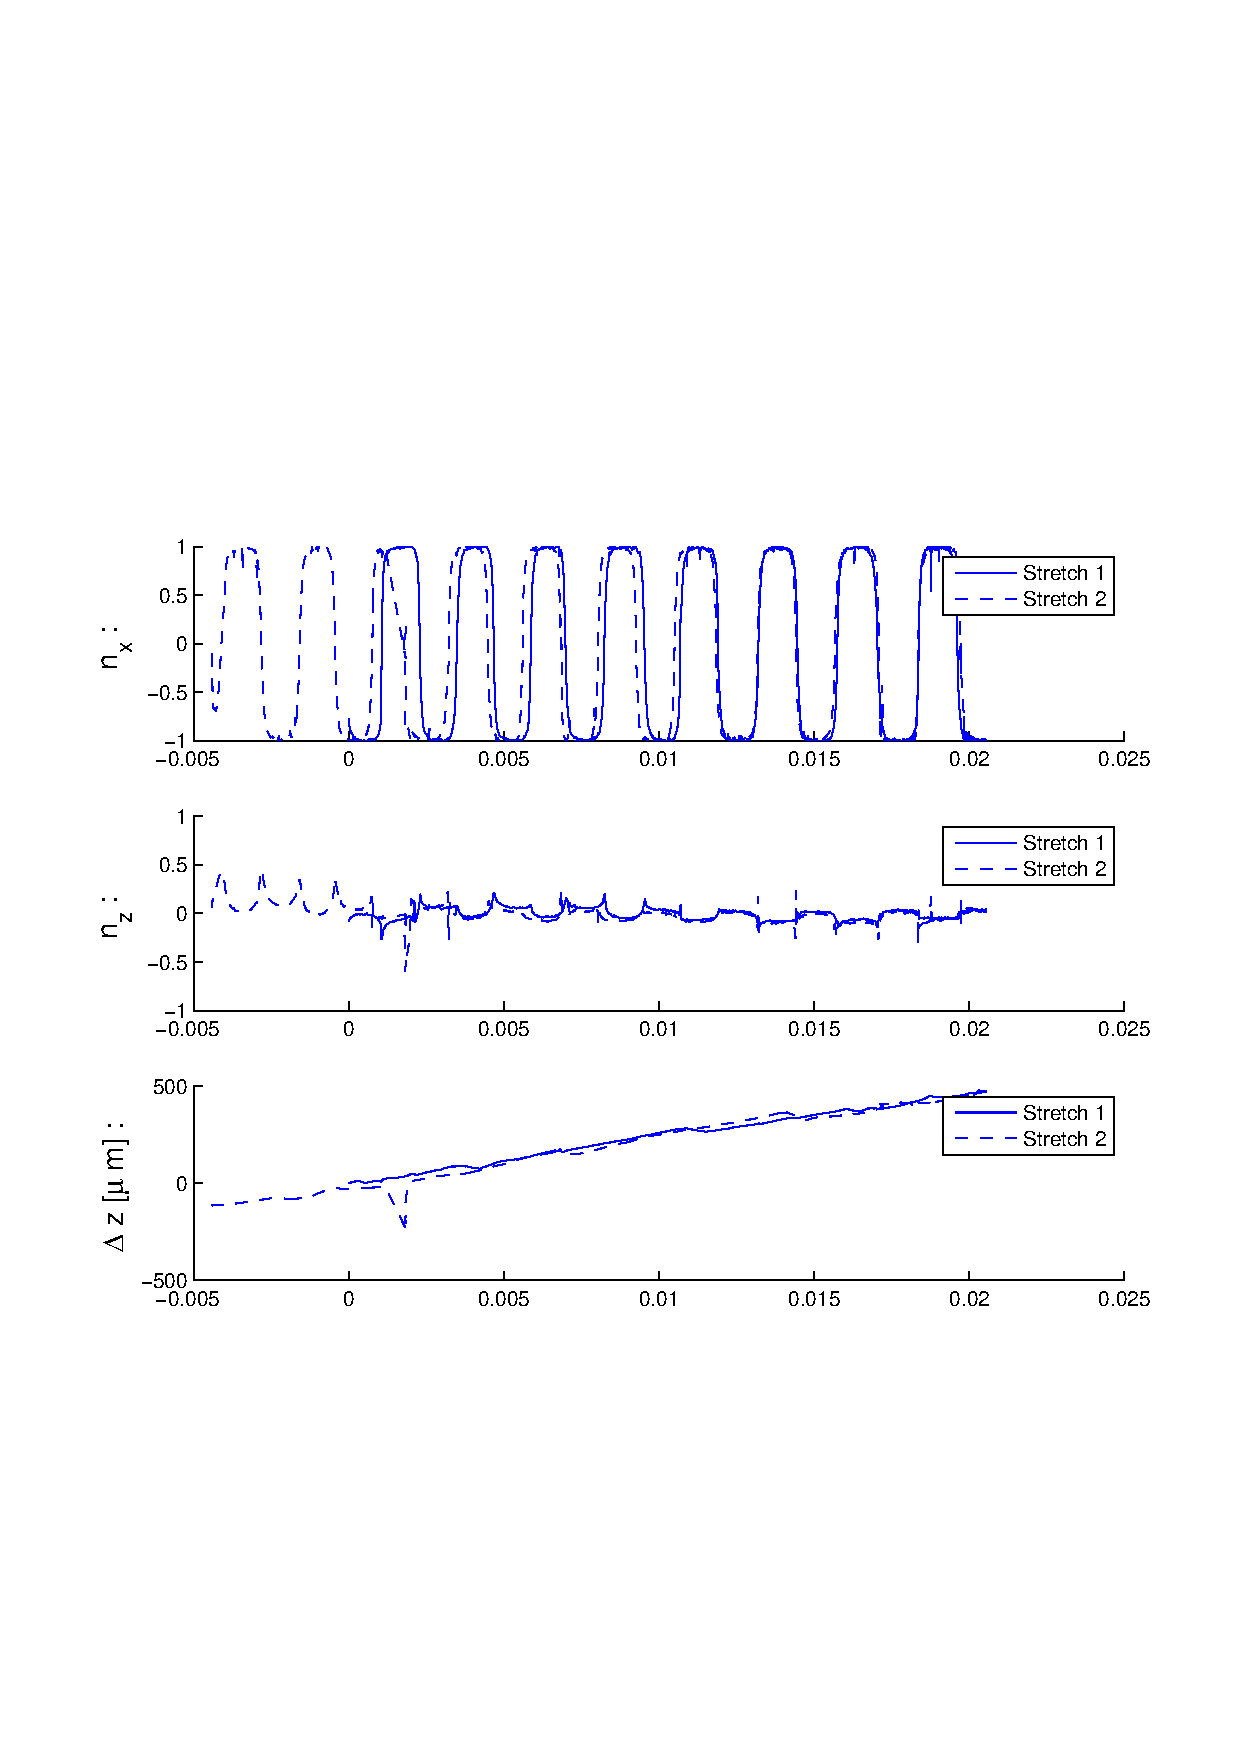
\includegraphics[width=0.8\textwidth]{Images/Particle 20/Stretch1.pdf}

\end{figure}



\subsection{Particle 24}

\begin{figure}[ H]

\caption{Particle 24: $ \lambda: 14.3715$Depth: 60 out of $200 \mu $ m}

\centering

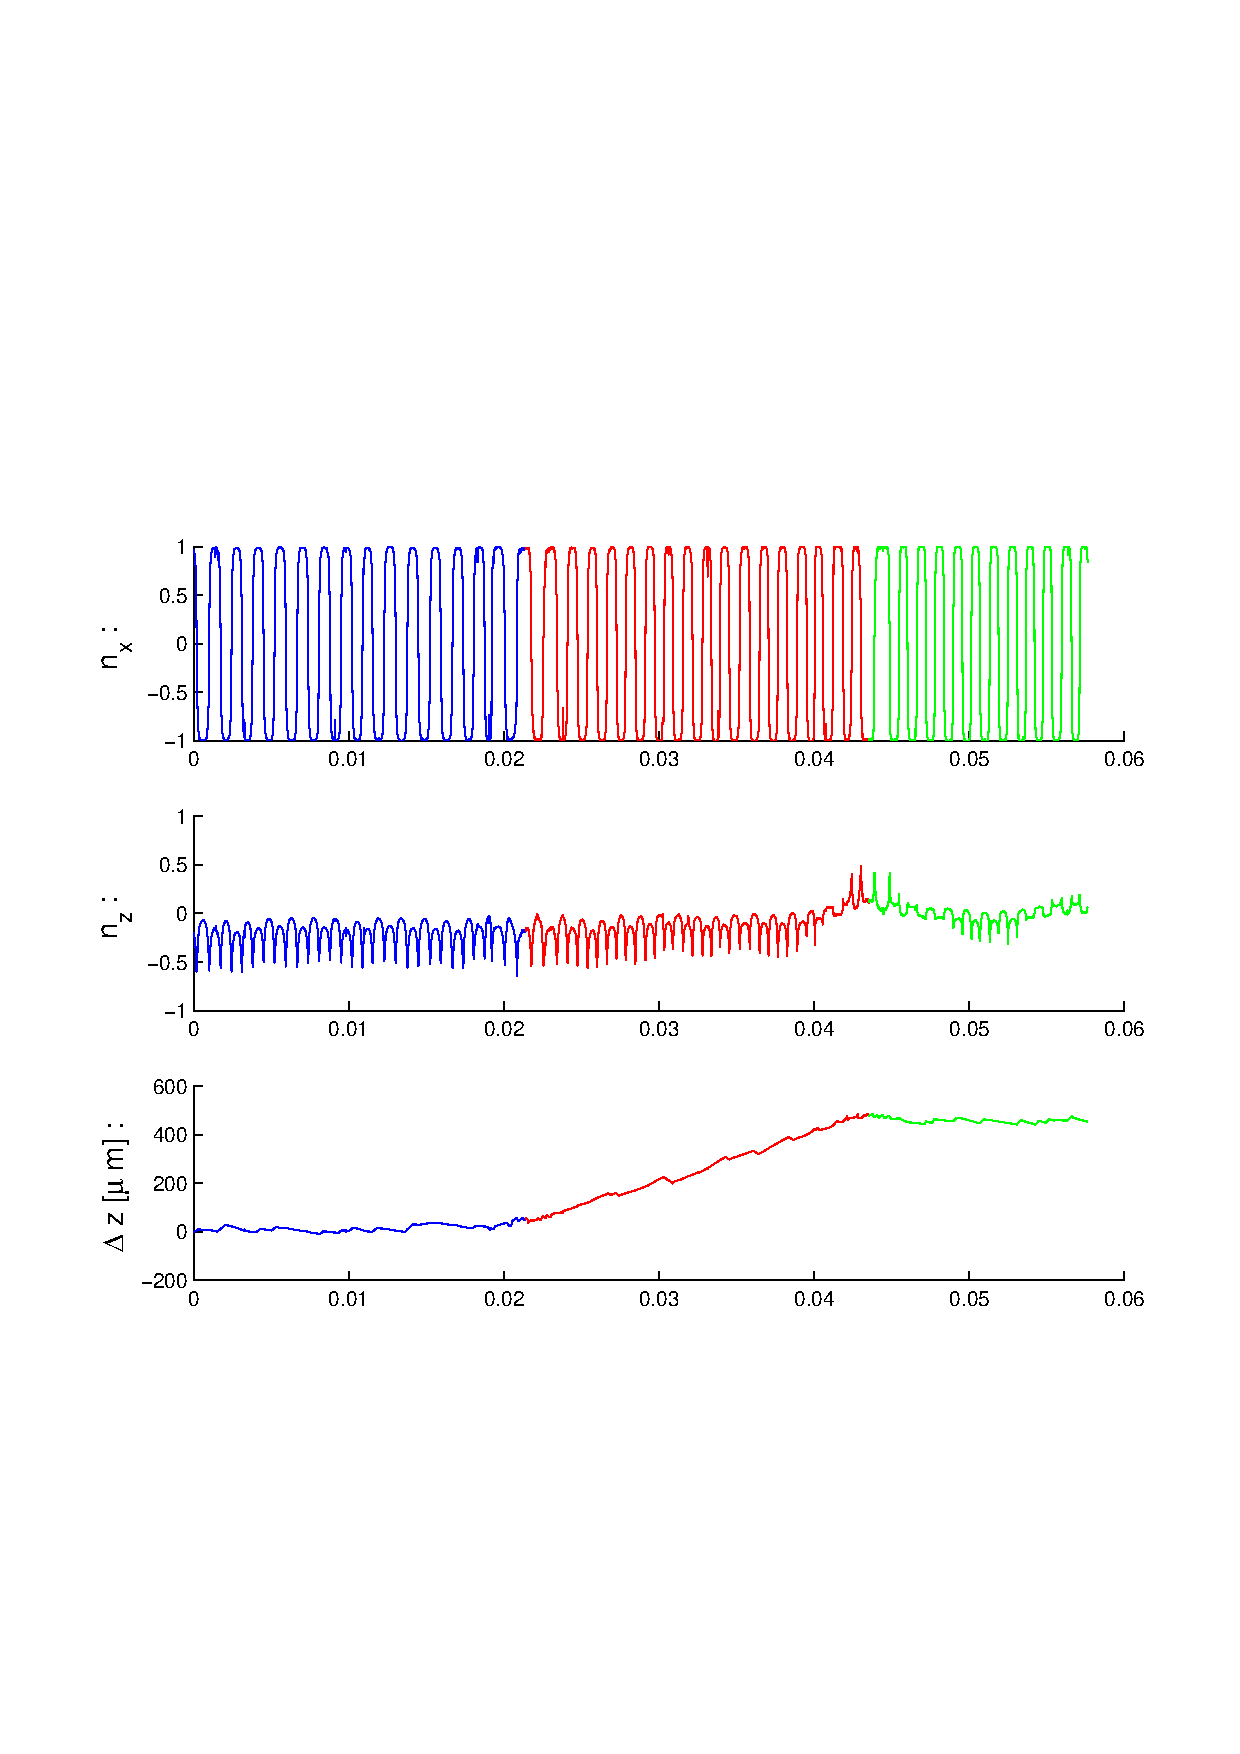
\includegraphics[width=0.8\textwidth]{Images/Particle 24/Particle24.pdf}

\end{figure}

\begin{figure}[ H]

\centering

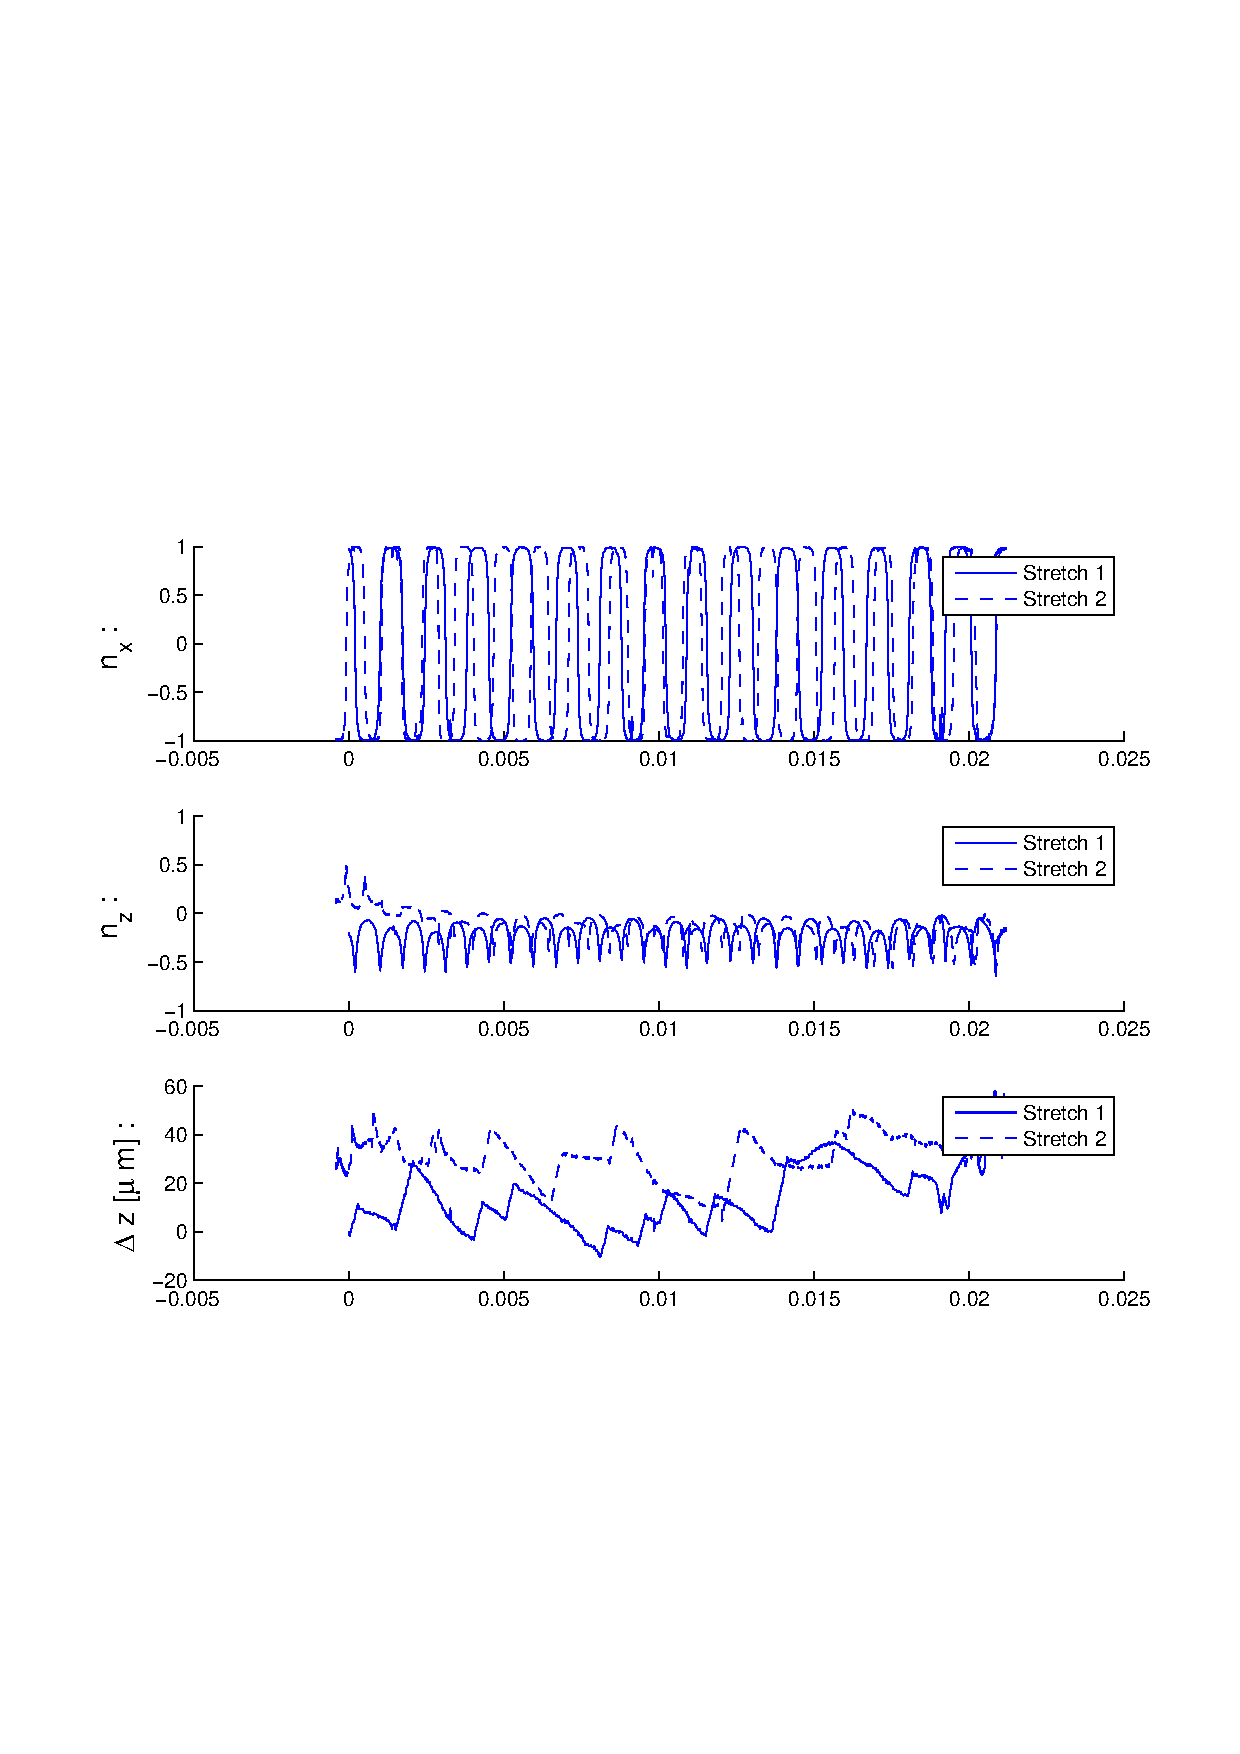
\includegraphics[width=0.8\textwidth]{Images/Particle 24/Stretch1.pdf}

\end{figure}

\begin{figure}[ H]

\centering

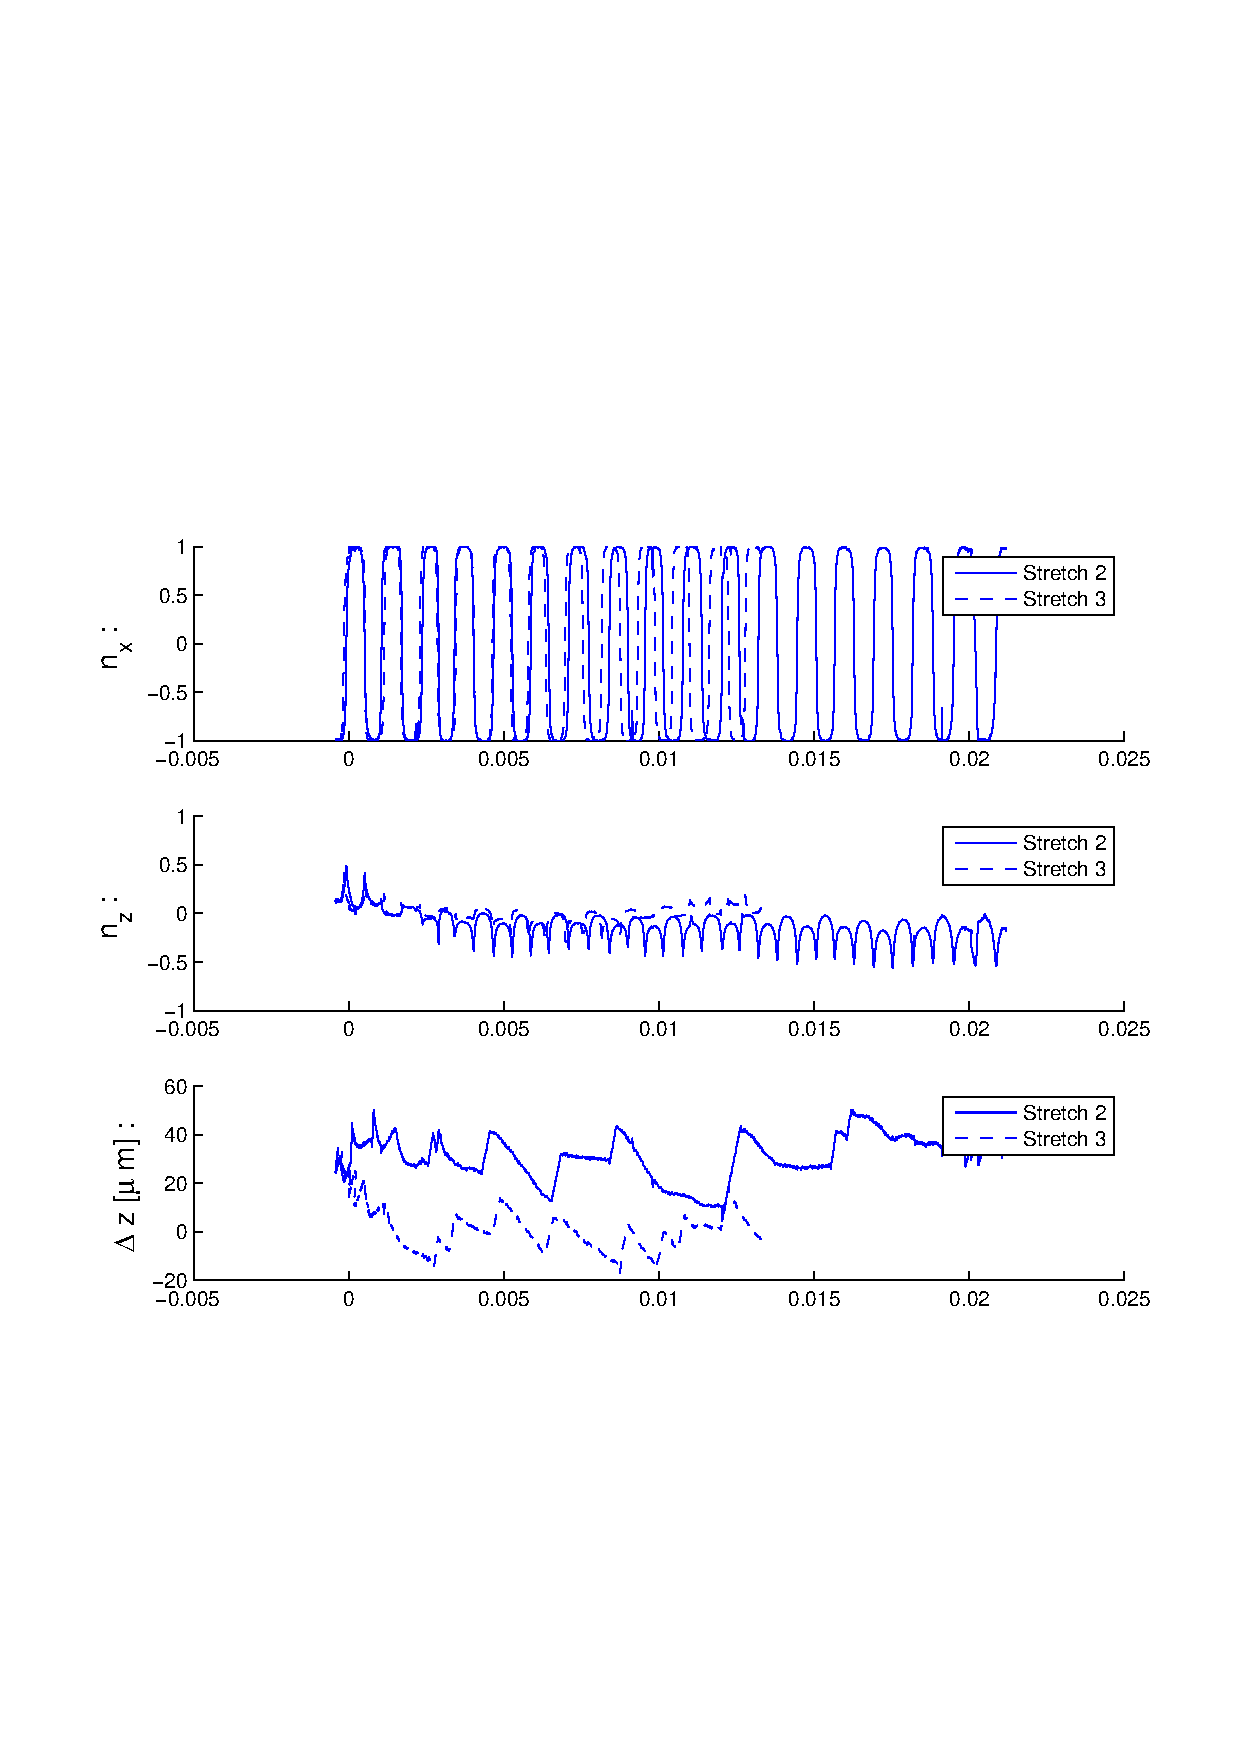
\includegraphics[width=0.8\textwidth]{Images/Particle 24/Stretch2.pdf}

\end{figure}
